\chapter{Reputation Availability}
\label{chap:rep_avail}
The incentive system's goal is to provide a good level of service to those peers
who abide by the rules of the system (TODO terminology: cooperating?). Since the
system measures this via a reputation point system, cooperating (TODO) peers
must be able to gain the required amount of reputation within a reasonable time
frame. At the same time, they should not be so quickly contented with their
level of reputation that they frequently lose the incentive to participate (TODO
are they still "cooperating" in this case?).

- being able to gain rep basically means being sent enough queries regularly

This chapter examines under which circumstances this is the case.

\section{Setup}
- TODO redo percentile graphs with all black lines, colors are meaningless
This chapter contains evaluations of many simulation runs. The
\texttt{.settings} (TODO link to section in implementation) files for
reproducing these results should be distributed along with this thesis in the
\texttt{thesis/simulation\_runs/} subdirectory. The \texttt{.settings} file name
for each result is given relative to that directory (TODO).

Most (TODO most or all?) of the simulation runs are based on the default
configuration (\texttt{default.settings} (TODO check that it's still current)).
For information on the meaning of the parameters, see the implementation chapter
(TODO link).

The most important parameters of the default settings are these (TODO move to
implementation, make into a table, explain the reason or significance of each
value):
\begin{itemize}
\item Random seed: 5803379951609632196
\item Number of peers: 64
\item Length of IDs: 16 bit
\item Length of routing prefixes: 4 bit (i.e. average sync group size of 4
      peers) (TODO this is just called "prefix" in the implementation, but
      "routing prefix" in the text to distinguish it from the general concept of
      a prefix)
\item Evenly sized sync groups are not ensured
\item Sync groups are ensured to be non-empty
\item Number of random introductions: 8
\item Subprefix coverage check interval: 10 seconds (TODO make sure it's clear
      what this is)
\item Sync peers are not queried when finding subprefix coverage (TODO
      terminology "finding coverage")
\item Maximum query group size: 16
\item Minimum desired number of query peers: 2
\item Reward for a successful query: 1 reputation point
\item Penalty for a failed query: 1 reputation point
\item Penalty for a timeout: 2 reputation points
\item No reputation decay
\item No-penalty reputation (TODO terminology): 10 reputation points
\item Request generation: 1 per second per peer (TODO possibly more complex
      request generation?)
\item Reputation attenuation: exponential with exponent 0.35, coefficient 1,
      lower bound 10 and upper bound 15
\item Transmission delay: 0.1 seconds
\item Network timeout: 2 seconds
\item Initial reputation: 0
\item Reputation buffer: 4 reputation points (meaning a tolerance of 2 timeout
      penalties (TODO still correct?))
\item Peer selection strategy: \emph{overlap $\rightarrow$ reputation sorted}
\item Group switching is disabled
\item Penalty expectations are enabled
\end{itemize}

Simulations usually (TODO usually or always?) last 200 seconds.

- TODO describe the peer behavior (get up to 14, let a timeout happen), or ref
  impl chapter

\section{Peer Selection Strategy}
\label{sec:selection}
Many requests or incoming queries make it necessary for a peer to send a query
to a query peer. The peer must then choose the recipient of the query. How peers
decide this influences the reputation availability in the system. 5 different
strategies have been implemented and are presented in the following.

- all peers use the same strategy
- should strategies not avoiding loops be penalized? (i.e. give penaltes for
  queries for target IDs to which the querying peer is closer than the queried
  peer)
- TODO find routing loops automatically
- TODO performance metrics for this chapter? e.g. average query time
- TODO new graph plotting how many query group memberships are above 10 rep, as
  a measure for rep gain ability (exclude very small groups?)
- TODO measure how often the recursive query problem occurs

\subsection{Strategy: \emph{Overlap}}
\label{sec:rep_avail_selection_overlap}
This is the default selection strategy that was described in the implementation
chapter (TODO link). Out of all possible recipients, the peer chooses one whose
routing prefix overlaps maximally with the target ID (TODO link overlap
definition in system description). Under the assumption that peers have complete
subprefix coverage, this ensures that queries always terminate and no routing
loops occur, since at each hop the distance to the target ID shrinks.

- TODO formalize overlap with target ID

The strategy does not specify a tie breaker. In the simulation query groups are
maintainer as Python \texttt{OrderedDict} objects, which are always iterated
over in a predictable order. Upon entering a query group, this object is copied
to the new member, so that he also has the same iteration order. This leads to a
problem where some "lucky" peers always get picked first, simply because of
their position in the dictionary. Others in contrast have a difficult time
getting any reputation because they don't receive queries (they may still
receive some, e.g.  after a peer let a query time out).

- TODO number of queries received histogram

Figure~\ref{fig:selection_overlap_peer_reps} shows examples of a peer (on the
left) who is "lucky" in one query group (not so much in others, but he can still
get by), and another (on the right) who is unable to gain sufficient reputation.
Other peers not shown are able to quickly gain reputation in all their groups.

An example of the effect on the reputation percentiles in a query group is shown
in figure~\ref{fig:selection_overlap_rep_percs}: the 50th percentile and above
can easily gain reputation, while peers below struggle.

(TODO recursive-query problem? peers who aren't getting queries can't answer the
ones they're getting in time. confirm.)

The underlying problem is that peers have no consideration for which peers could
use queries in order to gain reputation, nor do they have any incentive to.
There end up being "rich" peers and "poor" peers because of this.

While this is cause by an artifact of the implementation, it is by no means
certain that this problem couldn't occur in a real system. Peers may use an
implementation that also tends to favor some peers over others for lack of a tie
breaker.

\begin{figure}[t]
\centering
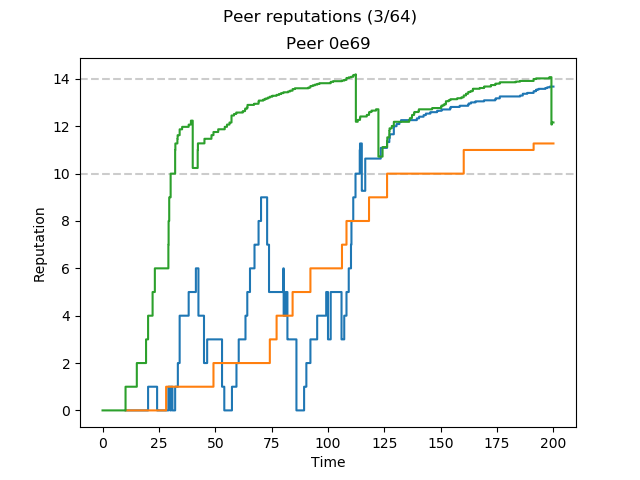
\includegraphics[width=0.5\columnwidth]{figures/selection_overlap_peer_reps_3_of_64}%
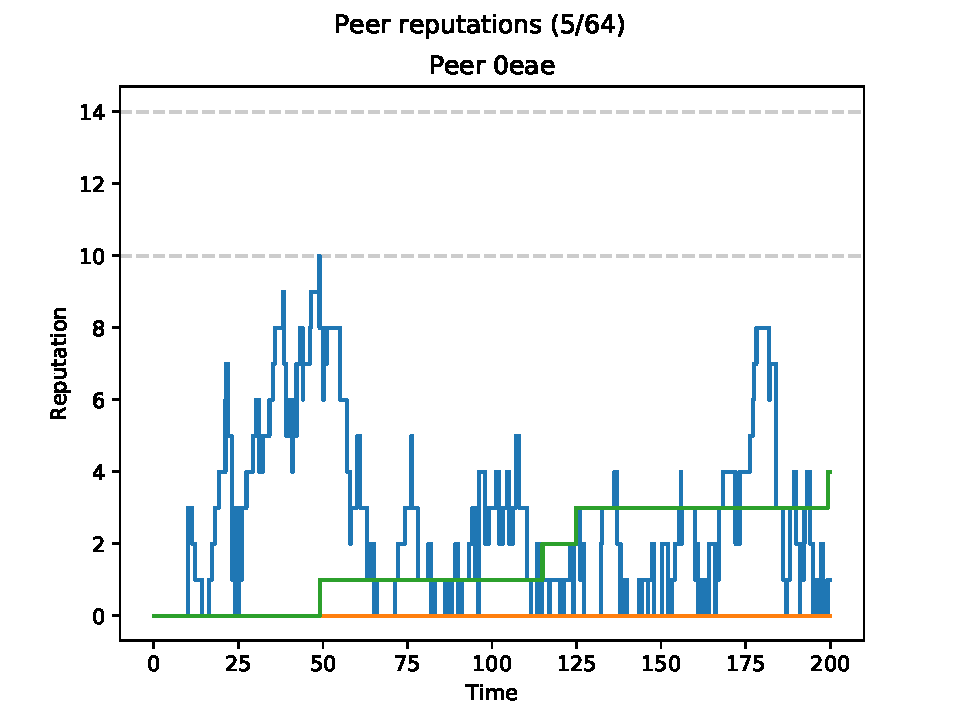
\includegraphics[width=0.5\columnwidth]{figures/selection_overlap_peer_reps_5_of_64}
\captionsettings{Reputation over time for strategy \emph{overlap} for 2
peers}{selection\_strategy/selection\_overlap.settings}
\label{fig:selection_overlap_peer_reps}
\end{figure}

\begin{figure}[t]
\centering
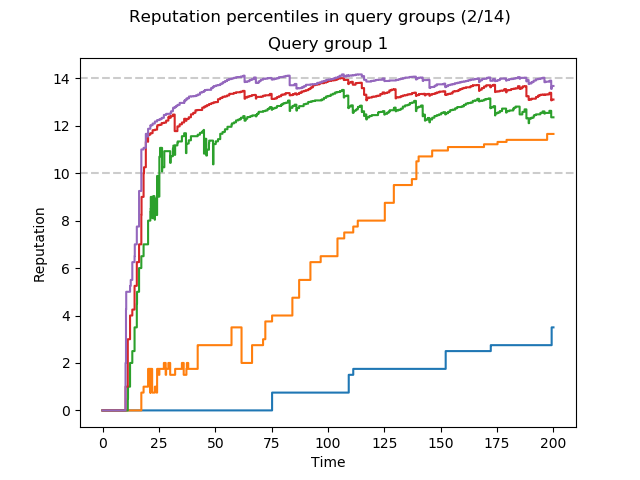
\includegraphics[width=1\columnwidth]{figures/selection_overlap_rep_percs_2_of_14}
\captionsettings{Reputation percentiles over time for strategy \emph{overlap} in
one query group}{selection\_strategy/selection\_overlap.settings}
\label{fig:selection_overlap_rep_percs}
\end{figure}

Figure~\ref{fig:selection_overlap_resp_statuses} shows the response statuses
over time. They are fairly well-behaved, with timeouts and unmatched responses
that settle at a low level.

\begin{figure}[t]
\centering
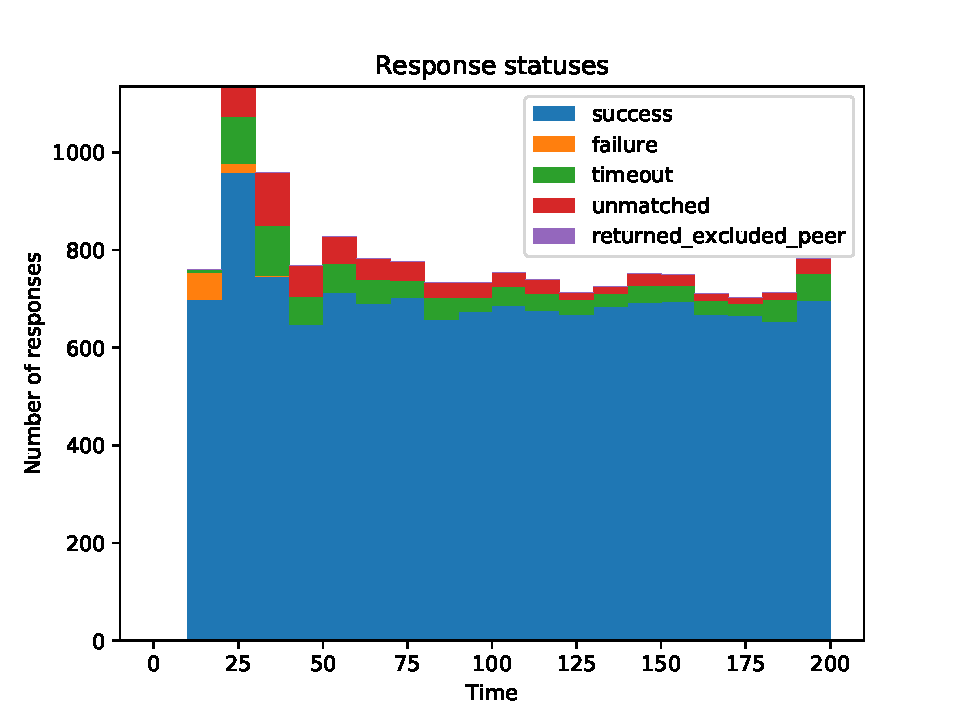
\includegraphics[width=1\columnwidth]{figures/selection_overlap_resp_statuses}
\captionsettings{Response statuses over time for strategy
\emph{overlap}}{selection\_strategy/selection\_overlap.settings}
\label{fig:selection_overlap_resp_statuses}
\end{figure}

- TODO interaction with attenuation, would be worse without

\subsection{Strategy: \emph{Overlap $\rightarrow$ Reputation Saturated Last}}
- TODO call the sending peer sender or querying peer for clarity?
This strategy is a modification of the \emph{overlap} strategy, but with a
secondary criterion as a tie breaker. Peers still start out choosing a recipient
based on the overlap of the recipient's routing prefix and the target ID, except
they give potential recipients who are \emph{reputation saturated} the lowest
priority.

The peer considers a potential recipient \emph{reputation saturated} if the
lowest reputation the potential recipient has in any query group shared with the
peer is greater or equal than the reputation at which the potential recipient
would let the query time out out of laziness. In the simulation, this is the
no-penalty reputation (TODO terminology) plus the reputation buffer.

Effectively, the peer makes a list of all known query peers (TODO only those he
hasn't queried before. make that clear, possibly somewhere before) and sorts it
by the overlap length, longest first. Then he goes through the list and takes
out any potential recipient who is reputation saturated and appends him to the
back. The peer at the beginning of the list is then chosen. That means that any
peer that is not reputation saturated will be chosen over peers that are.

The rationale behind this is that a reputation saturated recipient would not
bother responding, so the peer himself has an incentive not to choose that
recipient. As a side effect, it's supposed to shift queries away from those
peers that were chosen first with the \emph{overlap} strategy towards those who
were "unlucky".

The peer of course doesn't know exactly whether a potential recipient is
reputation saturated, since the amount of reputation at which he would stop
responding (if there is any) is a policy decision. But he can guess the
potential recipient's saturation reputation (TODO definition?), e.g. simply
taking his own. In the simulation, this is not a problem at all, since all peers
have the same reputation buffer.

- TODO number of queries received histogram

Rational choices for the saturation reputation are at discrete intervals and
correspond to the number of trembles a peer can tolerate. E.g., in the default
settings, the reputation buffer is 4, for a total of 14 reputation, which allows
a peer to let one query time out for a penalty of 2 and still have 12
reputation. An unintentional timeout after that would leave the peer still at or
above the 10 no-penalty (TODO terminology) reputation. Another rational choice
would be a reputation buffer of 3, which would allow a peer to tolerate a failed
query penalty (of 1). But a reputation buffer of e.g. 3.5 doesn't make sense,
since it doesn't give the peer a possibility he wouldn't have with a buffer of
3 (there is no penalty of 1.5 in the rules). So the peer has some indication
about what assumption to make about the potential recipients reputation
saturation. (TODO this entire paragraph isn't completely accurate. a peer could
want to be able to tolerate one tremble and then already have some reputation
above 10 to get back to 12 in a shorter time, perhaps based on experience with
his average tremble rate and reputation gain rate)

Since this strategy is based on the \emph{overlap} strategy, it also protects
against routing loops under the previous assumption that the querying peer has
complete subprefix coverage, with the added stipulation that not all peers with
a higher overlap (of which there must be at least one since the peer has
complete subprefix coverage) are sorted to the back. If they are, routing loops
may occur, where the query gets forwarded to someone further from the target and
eventually back to the peer who issued it in the first place. That peer will
then wait for the response to his first query to answer that same query that
looped back around to him, which, of course, will never arrive. Eventually, the
timeout on the initial query kicks in, and penalties are applied, possibly even
along the loop, so that the peer who initiated the first query is penalized for
essentially not answering his own query (TODO confirm). The peer will eventually
try the reputation saturated peers closer to the target. However, these then may
choose to query peers further away from the target, leading to a new routing
loop, and fail to respond in time. In effect, this can contribute to queries not
being answered at all.

- check notes for interpretation. still same conclusions, or has some change in
  the simulation altered the results?

Figure~\ref{fig:selection_overlap_high_rep_last_rep_percs} shows the reputation
percentiles of 2 query groups. The ability for peers of the lowest percentiles
to gain reputation compares favorably to the \emph{overlap} strategy, they are
able to eventually pass the no-penalty reputation. However, they take much
longer to do it than peers of the higher percentiles. Both of these observations
were to be expected, since "unlucky" peers (who previously were not selected
first due to their position in the iteration order) are now given priority once
the "lucky" ones are reputation saturated.  But this takes time, explaining the
delay for the lower percentiles.

\begin{figure}[t]
\centering
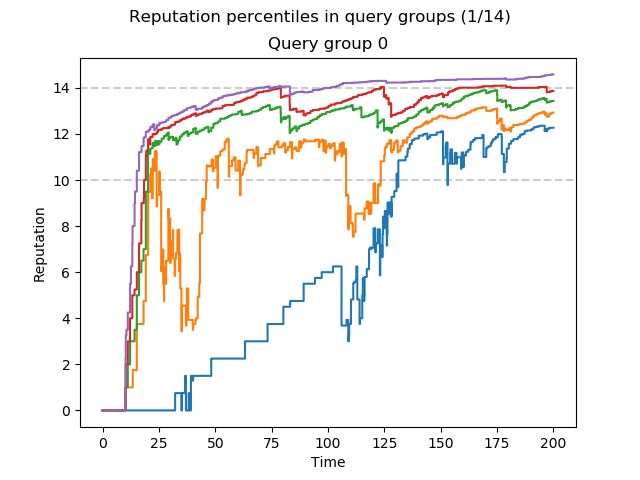
\includegraphics[width=0.5\columnwidth]{figures/selection_overlap_high_rep_last_rep_percs_1_of_14}%
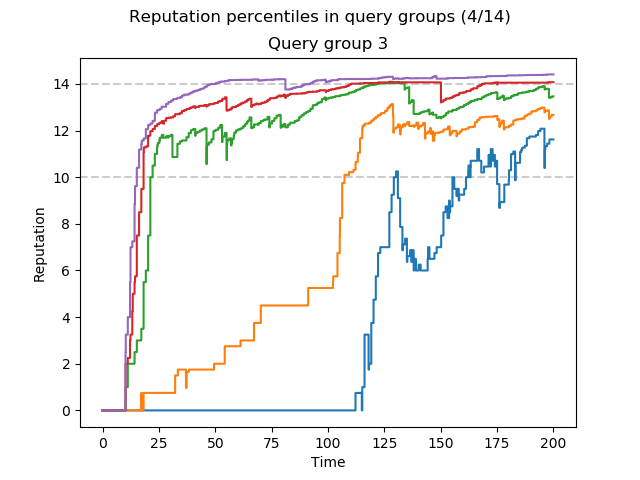
\includegraphics[width=0.5\columnwidth]{figures/selection_overlap_high_rep_last_rep_percs_4_of_14}
\captionsettings{Reputation percentiles over time for strategy \emph{overlap
$\rightarrow$ reputation saturated last} in 2 query
groups}{selection\_strategy/selection\_overlap\_high\_rep\_last.settings}
\label{fig:selection_overlap_high_rep_last_rep_percs}
\end{figure}

Figure~\ref{fig:selection_overlap_high_rep_last_peer_reps} shows the reputation
development of 2 peers. On the left, an example of a peer gaining quickly in one
group, but with a delay in another. On the right, an extreme example for whom
reputation gains in all groups is delayed for a long time, but happens
eventually. There are also examples of peers able to gain reputation quickly in
all groups not shown here.

\begin{figure}[t]
\centering
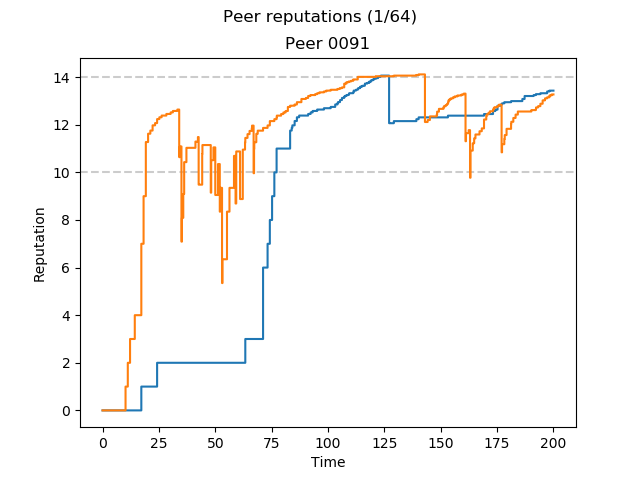
\includegraphics[width=0.5\columnwidth]{figures/selection_overlap_high_rep_last_peer_reps_1_of_64}%
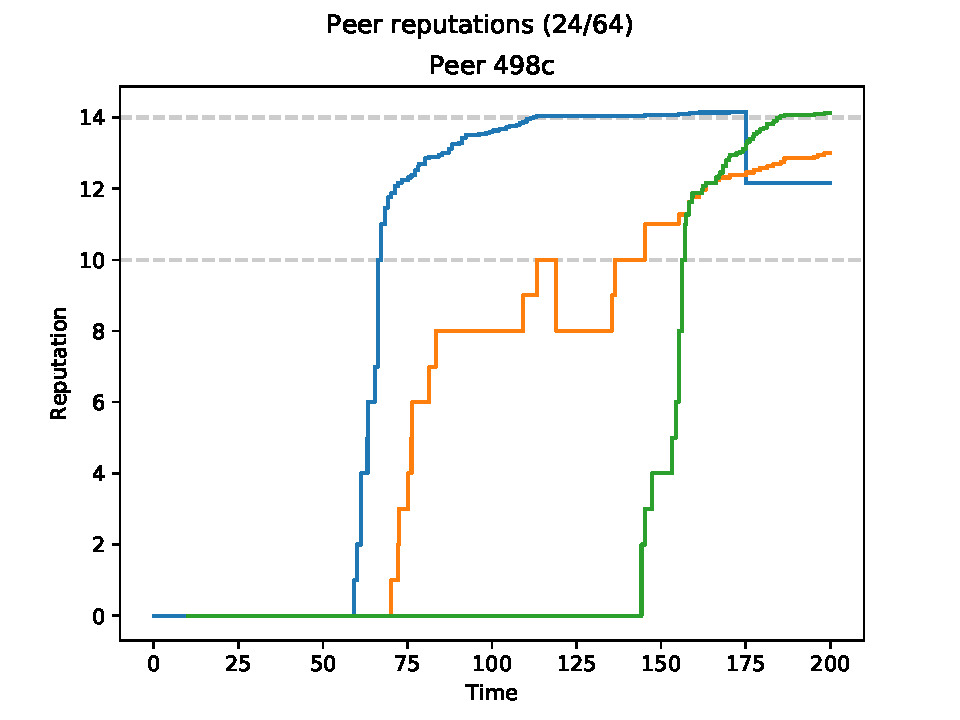
\includegraphics[width=0.5\columnwidth]{figures/selection_overlap_high_rep_last_peer_reps_24_of_64}
\captionsettings{Reputation over time for strategy \emph{overlap $\rightarrow$
reputation saturated last} for 2
peers}{selection\_strategy/selection\_overlap\_high\_rep\_last.settings}
\label{fig:selection_overlap_high_rep_last_peer_reps}
\end{figure}

- TODO compare response statuses in a more systematic manner (and include number
  of responses)

Figure~\ref{fig:selection_overlap_high_rep_last_resp_statuses} shows the
response statuses over time. Compared with the \emph{overlap} strategy, there
are a few more timeouts and unmatched queries. The difference isn't big, but can
be explained by the possibility of selecting unsuitable peers. The possibility
of routing loops was discussed, but they may also happen if queries are sent to
recipients suffering from the recursive query problem (TODO terminology). (TODO
confirm from the log)

\begin{figure}[t]
\centering
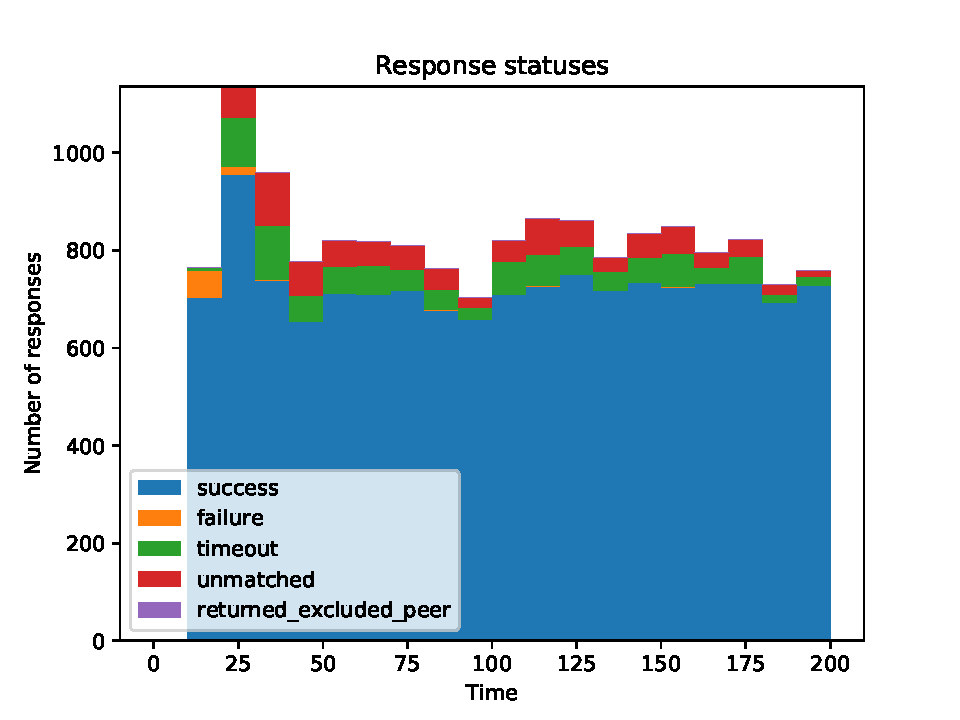
\includegraphics[width=1\columnwidth]{figures/selection_overlap_high_rep_last_resp_statuses}
\captionsettings{Response statuses over time for strategy \emph{overlap
$\rightarrow$ reputation saturated
last}}{selection\_strategy/selection\_overlap\_high\_rep\_last.settings}
\label{fig:selection_overlap_high_rep_last_resp_statuses}
\end{figure}

\subsection{Strategy: \emph{Overlap $\rightarrow$ Reputation Sorted}}
\label{sec:rep_avail_selection_overlap_rep_sorted}
This strategy is another modification of the \emph{overlap} strategy. The
querying peer again takes all viable query peers (i.e. those that haven't been
queried for the target ID already) and sorts them by the length of the overlap
of their routing prefix with the target ID, longest first. As a secondary
sorting criterion he uses the reputation the potential recipient has in any
shared query group (TODO find a term for this, see definitions in system
description chapter), lowest first. So effectively, out of all potential
recipients he will only consider the subset consisting of those whose overlap is
greatest and chose the one with the lowest reputation.

The strategy was designed to address the issue with \emph{overlap $\rightarrow$
reputation saturated last}, namely that "unlucky" peers still have to wait for
the "lucky" ones to become reputation saturated before they can gain reputation
at a practical rate. With that, it was left up to chance whether a peer could do
well in the system, which is not a desirable property because it could scare off
potentially valuable contributors.

By selecting the lowest-reputation peer (within the group with maximal overlap),
the ability to gain reputation is supposed to be better distributed among all
peers. It is of course still required for a peer to be useful to others in the
query group, i.e. to serve a routing prefix subprefixes of which others query
for (longer ones are better). This is what leads to the peer being in the group
of considered peers with maximal overlap in the first place (TODO mention group
switching section here?).

- TODO number of queries received histogram

- attenuation means it takes a lot longer to get from 10 to 14 than from 0 to
  10. that means socially it is better that all gain at the same rate (e.g.
  unlucky peers shouldn't have to wait for lucky ones to be rep saturated),
  since that's the quickes way to get everyone penalty-free

Figure~\ref{fig:selection_overlap_rep_sorted_rep_percs} shows reputation
percentiles in 2 query groups. One in which reputation is gained easily gained
by all peers, one in which the 5th percentile can't quite maintain the
no-penalty reputation for a while (TODO likely from recursive query problem,
with one peer in a small query group where getting to 10 takes a long time.
check that) (TODO clarify that this is good).

\begin{figure}[t]
\centering
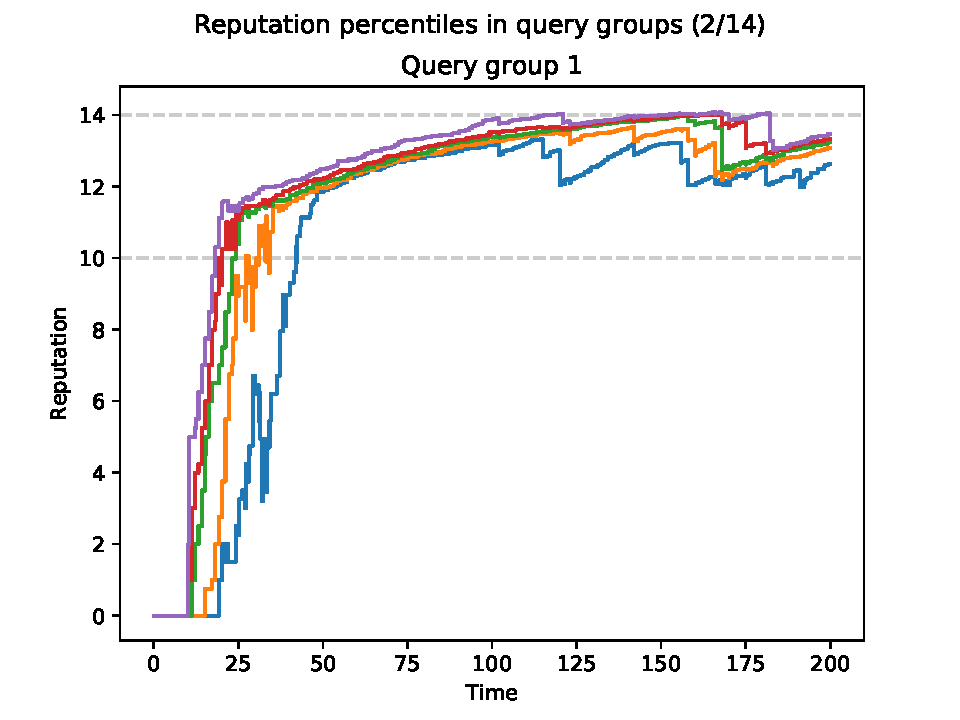
\includegraphics[width=0.5\columnwidth]{figures/selection_overlap_rep_sorted_rep_percs_2_of_14}%
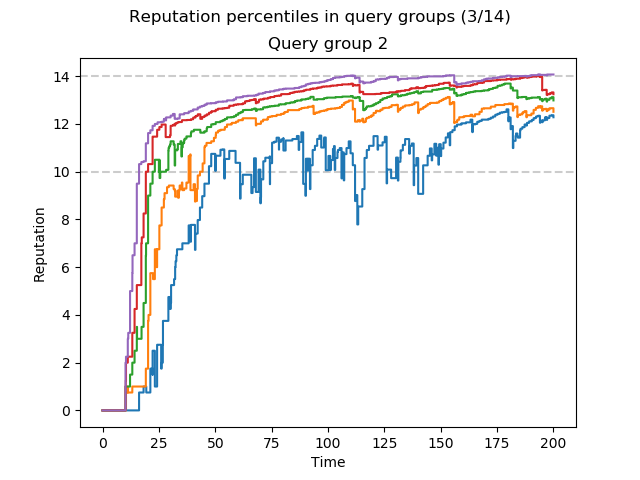
\includegraphics[width=0.5\columnwidth]{figures/selection_overlap_rep_sorted_rep_percs_3_of_14}
\captionsettings{Reputation percentiles over time for strategy \emph{overlap
$\rightarrow$ reputation sorted} in 2 query
groups}{selection\_strategy/selection\_overlap\_rep\_sorted.settings}
\label{fig:selection_overlap_rep_sorted_rep_percs}
\end{figure}

Figure~\ref{fig:selection_overlap_rep_sorted_peer_reps} shows the reputation
development of 2 peers. The one on the left has it very easy to gain reputation,
the one on the right struggles for a while in 2 of his 3 query groups, but can
eventually gain and maintain beyond the no-penalty reputation. This is about the
worst case as well (TODO excluding peers in very small groups).

The left graph very clearly shows a sort of sawtooth pattern that stems from the
peer letting a query time out once he is reputation saturated at 14 reputation,
thus falling dow to 12 and subsequently starting to gain reputation again.

\begin{figure}[t]
\centering
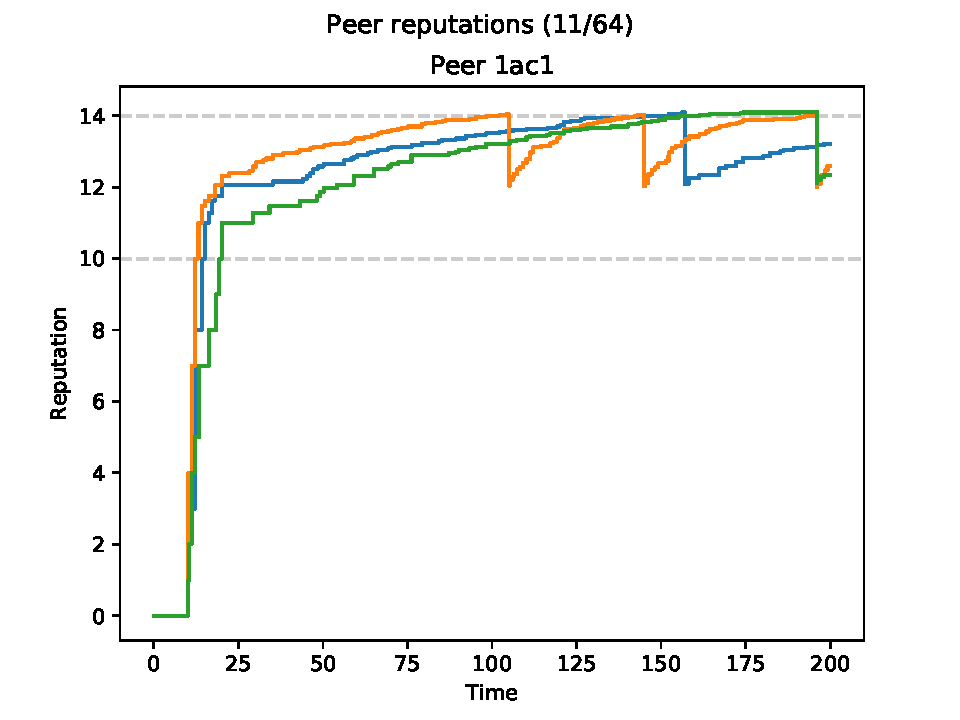
\includegraphics[width=0.5\columnwidth]{figures/selection_overlap_rep_sorted_peer_reps_11_of_64}%
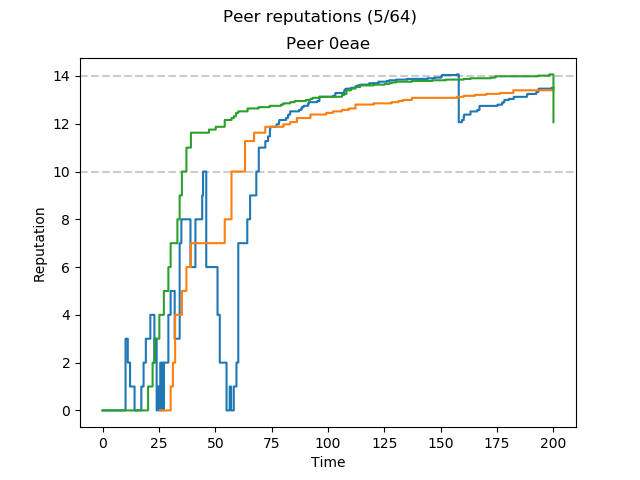
\includegraphics[width=0.5\columnwidth]{figures/selection_overlap_rep_sorted_peer_reps_5_of_64}
\captionsettings{Reputation over time for strategy \emph{overlap $\rightarrow$
reputation sorted} for 2
peers}{selection\_strategy/selection\_overlap\_rep\_sorted.settings}
\label{fig:selection_overlap_rep_sorted_peer_reps}
\end{figure}

The frequencies of response statuses presented in
figure~\ref{fig:selection_overlap_rep_sorted_resp_statuses} shows this
strategy to be better than the other \emph{overlap} strategies in terms of query
success rate. The fact that peers can quickly gain reputation and receive
penalty-free service makes the recursive query problem (TODO terminology) less
likely (TODO confirm by measuring how often it happens), leading to fewer
timeouts.

\begin{figure}[t]
\centering
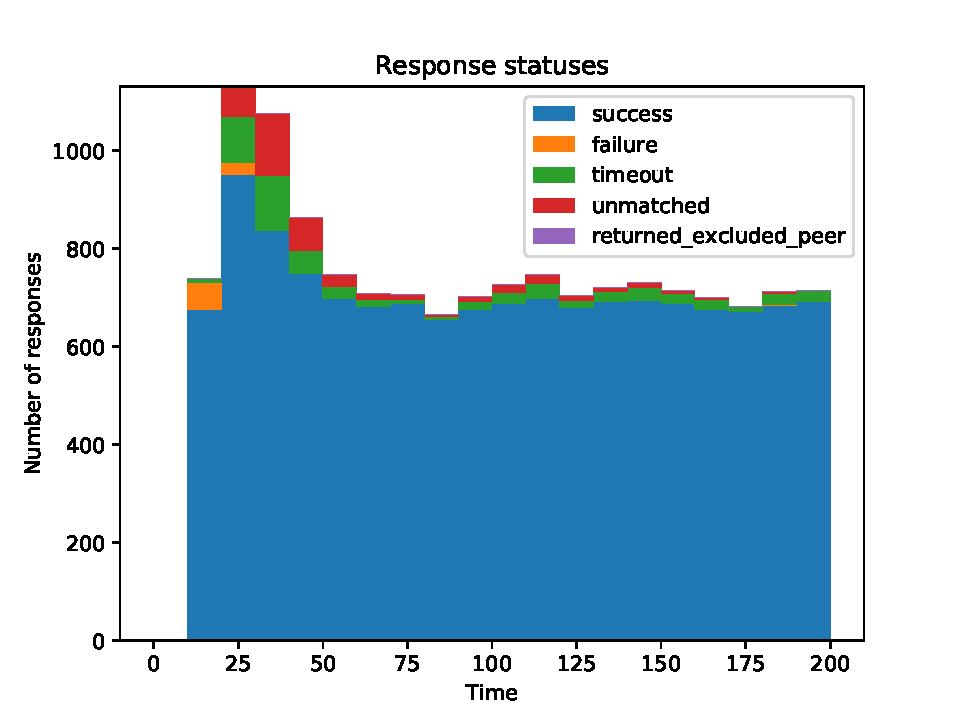
\includegraphics[width=1\columnwidth]{figures/selection_overlap_rep_sorted_resp_statuses}
\captionsettings{Response statuses over time for strategy \emph{overlap
$\rightarrow$ reputation
sorted}}{selection\_strategy/selection\_overlap\_rep\_sorted.settings}
\label{fig:selection_overlap_rep_sorted_resp_statuses}
\end{figure}

\emph{Overlap $\rightarrow$ reputation sorted} is the best performing of the
strategies presented here for the purpose of reputation availability.
Essentially all peers can quickly and reliably gain reputation (TODO not in
small groups, but that's a problem with the implementation).

It also prevents routing loops as well as any, since the querying peer always
picks a recipient from the group of peers with maximal overlap. In this regard,
it is clearly better than \emph{overlap $\rightarrow$ reputation saturated
last}, where this was not necessarily the case.

- TODO abbreviations? lrp - lowest-rep peer, qp - querying peer, ar - actual
  recipient, etc.

\subsubsection{Contented Peers}
\label{sec:rep_avail_selection_rep_sorted_contented}
It must be pointed out that, in the simulation, all peers are willing to
contribute for the best possible service, i.e. they do their best to answer
queries until they are reputation saturated (TODO this assumption should have
been stated in a previous chapter, description or implementation). Any peers who
are not contributing because they are contented with the lowest level of service
(called \emph{contented peers} for this discussion) would remain at 0
reputation.  They would thus be strongly favored for selection, but the effort
wasted on them, and queries remain unanswered.

This could have desastrous results on overall performance for queries where the
group of peers with maximal overlap contains a contented peer. Firstly, in the
case where querying peers only send one query, the first query is always going
to fail, adding a timeout to the total lookup time.

Secondly, in case the querying peer sends two (or more) queries, the one
addressed to the contented peer is wasted; it was meant to allow the
lowest-reputation peer to gain reputation, but this opportunity is given to the
contented peer, who will not seize it. In this case, the purpose of this
selection strategy, to enable low-reputation peers to get started and in effect
to increase social value, is not served.

- TODO do a simulation with contented peers

Possible solutions to this problem could be based on treating the contented peer
differently from the other peers. First, this requires detecting that the peer
is indeed contented. If he is nice, he could announce this upon joining the
group (he may still be tolerated in the group if he gives rewards for successful
queries). If he isn't, detection would have to be based on experience: a peer
who never responds to queries is potentially contented.

- TODO is there really incentive to try to detect contented peers? what's the
  immediate benefit for the peer for going through that trouble?

Once there is a suspicion that a peer is contented, he, and any other contented
peers, can be skipped when selecting peers. That is, when making the list of
viable potential recipients, contented peers are excluded. If the peer really is
contented, he shouldn't mind not receiving the query, and certainly not
complain, out of laziness (if he does complain, he would be better classified as
malicious, since he takes action that is not to his own benefit, but to the
detriment of the group).

Contented peers who are so lazy they don't even bother giving rewards for
succesful responses they received could be dealt with via the complaint system
or the query group management (TODO ref system description). Peers who should
have gotten a reward but didn't can complain or just make an effort to have the
peer removed from the group.

\subsubsection{Enforcement}
\label{sec:selection_overlap_rep_sorted_enforcement}
The downside of this strategy is that there is no inherent incentive for peers
to use it. It may provide good social value, but for any individual choice a
querying peer could decide that the lowest-reputation peer is less likely to
answer, or likely to take more time, than some other one. This could be from
previous experience, or from the assumption that a peer with low reputation in
one query group also has low reputation in other query groups, leading to the
recursive query problem (TODO terminology) and longer response times.

So in order for this strategy to be implemented in a real system, the rules of
the system must make querying the lowest-reputation peer mandatory. The querying
peer may send multiple queries, but for any query group he shares with the
recipient of a query, the lowest-reputation peer in that query group with
maximal overlap must also be sent one. A behavior conformant with this rule
would be for the querying peer to use whatever criteria he wishes to select the
recipient, and then to additionally query the lowest-reputation peer.

This rule has to be enforced to be useful. The enforcement process encompasses
two things: detecting that the querying peer failed to also send a query to the
lowest-reputation peer, and agreeing whether a penalty should be applied to the
querying peer and a compensation to the lowest-reputation peer.

The first of these problems may be tackled in one of two ways: the
lowest-reputation could monitor reputation updates in the query group. He then
knows a querying peer failed to send him a query if there is a reward or penalty
applied by the querying peer to some other peer for a query the
lowest-reputation peer should also have received but didn't. This requires
reputation updates regarding responses to include which target ID they're about.
However, this has privacy implications (see
\ref{sec:selection_overlap_rep_sorted_privacy}), and there is neither any
incentive for the querying peer sending the reputation update to include
truthful information and thus risk a penalty, nor is there any incentive for the
subject of the reputation update (the one being given a reward or penalty) to
correct false information. Since no one else knows the truth about the target
ID, this approach is not promising.

The other approach to detecting missing queries to the lowest-reputation peer is
to let all recipients of queries check if there is another peer in the query
group with equally large overlap, but less reputation than them. The actual
recipient of a query has all the necessary information and so could raise this
issue. Then, if this leads to the lowest-reputation peer receiving compensation,
the actual recipient would receive a reward as well, as a sort of finder's fee
to incentivize the checking.

This approach can cause trouble in the presence of contented peers. The proposed
solution to dealing with those was to ignore them and not send them queries. But
if another peer then notices this and starts the enforcement process, the
querying peer may end up being penalized. This brings back all the problems of
contented peers blocking actually contributing peers from gaining reputation. A
possible modification of the enforcement could require the lowest-reputation
peer (the contented peer in this case) to make the complaint himself. Under the
assumption that the contented peer truly is contented, he would be too lazy to
even do that. In addition, if the actual recipient of the query who noticed the
lacking query to the lowest-reputation peer is aware that he is contented, he
need not bother informing him, since there is no hope of a finder's fee anyway.

The second stage of enforcement is coming to an agreement whether a penalty
should be applied to the querying peer and compensation awarded to the
lowest-reputation peer. This must be done via the complaint system (TODO ref),
since no other than the two peers involved know the truth about whether a query
was sent. And in case the querying peer sends a reputation update without ever
sending a query to make his failure to send the query not-detectable by the
actual recipient, this is also a case for the complaint system (TODO does this
work even if he sends a reward? does the low-rep peer have an incentive to
complain?).

To clarify, this system has not been implemented in the simulation.

- TODO implement this, or a simplified version, for the next chapter?

\subsubsection{Privacy Implications}
\label{sec:selection_overlap_rep_sorted_privacy}
Employing this strategy has privacy implications. The entire point of the
reputation system is to incentivize participation in order to give each peer
many choices where to forward queries to and thus make profile building harder
(TODO wording: spread yourself thin or something).

This strategy demands that a querying peer tell one other specific peer (the
lowest-reputation peer) which target ID he is interested in. But the querying
peer may not want to do that, for whatever reason. Maybe he doesn't trust the
peer (from previous experience, maybe he believes he is being followed), maybe
he has already sent him plenty of queries in the past and doesn't want him to
have too much information (see section~\ref{sec:desc_stalking}).

Peers who are very sensitive to this could of course be in many more query
groups than is required for subprefix coverage, giving them a wider choice of
peers to query and making it less likely they feel forced into a bad situation.

A modification alleviating this issue is to only require a peer to query the
lowest-reputation peer if he has less than the no-penalty reputation (getting
everyone above that threshold quickly is the purpose of the strategy, after
all). Assuming that peers generally do well, this would further reduce the
number of instances of having to send unwanted queries.

There is another issue that was mentioned in
\ref{sec:selection_overlap_rep_sorted_enforcement}: if reputation updates
regarding responses must include the target ID, this is equivalent to
broadcasting to the entire query group the target ID of each query, a much more
severe infringement than the one described. Sure enough, for that purpose (to
detect whether a query should also have been sent to the lowest-reputation
peer) it would be enough to include only the routing prefix of the target ID,
but this still leaks a lot of information. Luckily, the approach that required
this has an alternative and wasn't very promising anyway.

\subsubsection{Possible Impact on Usefulness}
- does this maybe remove incentive to find a query group in which one is useful
  (since the system guarantees some queries)? peers may only be good for one
  subprefix, but are getting all the queries for it
- ref query group reevaluation section, explain what usefulness is (already done
  in system description)
- hasn't been implemented, not clear

\subsection{Strategy: \emph{Reputation Sorted}}
- no routing loop protection
\subsection{Strategy: \emph{Random}}
- no routing loop protection
- time it takes to get to no-penalty rep, dependent on who gets picked first
- impact of allowing to not use maximal overlap peers: hop count, timeouts (due
  to penalties, recursive queries), failures?
\subsection{Uneven Query Distribution}

\section{Reputation Decay}
- decay, necessary (see system description), but difficult
- decay doesn't really work if it's supposed to be the main incentive in
  continuing to participate: too difficult to balance even with the constant
  stream of requests; need timeout penalties as main measure
- possible solutions: vary decay rate with total reputation in group, or with
  average number of queries in a group or something
- describe how it would be implemented

\section{Penalty Expectations}
\label{sec:penalty_expectations}
Reputation attenuation, introduced in section~\ref{sec:attenuation}, as well as
penalty expectations, introduced in this section, are enabled in the default
settings. When both are disabled, quite severe oscillations in individual peer
reputations can be observed that are also reflected in reputation percentiles of
query groups.

\begin{figure}[t]
\centering
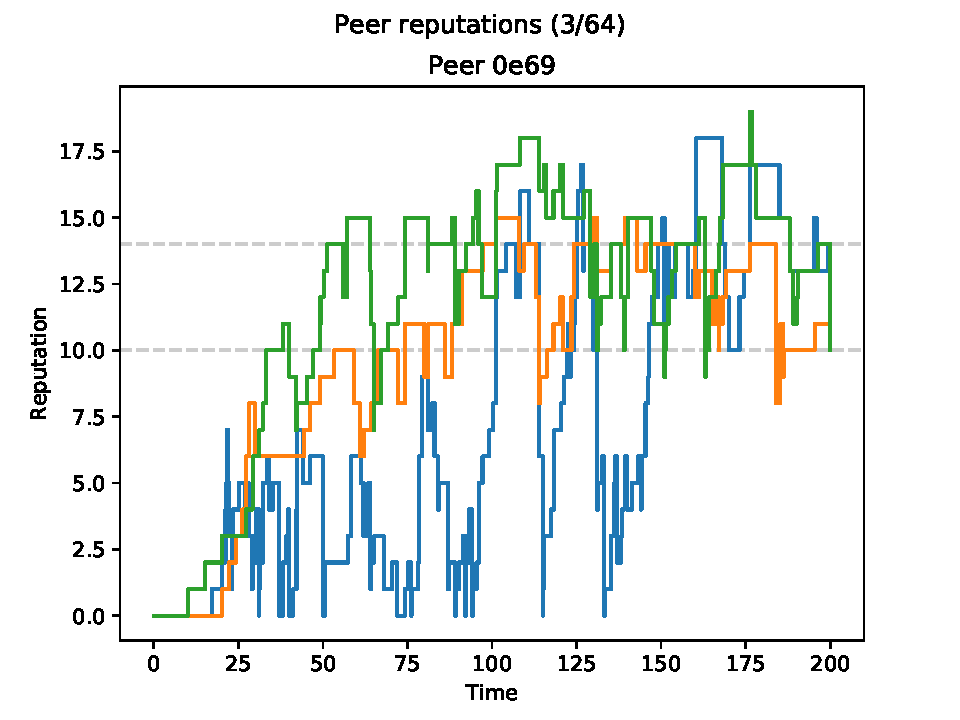
\includegraphics[width=0.5\columnwidth]{figures/expectations_off_no_att_peer_reps_3_of_64}%
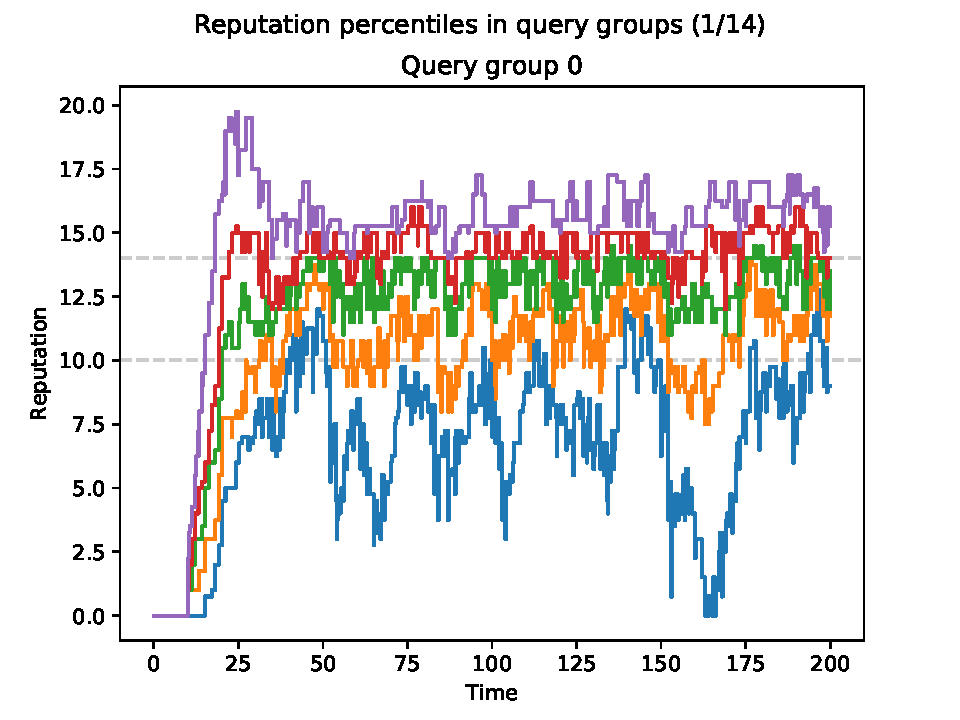
\includegraphics[width=0.5\columnwidth]{figures/expectations_off_no_att_rep_percs_1_of_14}
\captionsettings{Reputation oscillation of a peer and in the percentiles of a
query group with penalty expectations and reputation attenuation
off}{penalty\_expectations/expectations\_off\_no\_att.settings}
\label{fig:penalty_expectations_off_no_att_peer_reps_percs}
\end{figure}

Figure~\ref{fig:penalty_expectations_off_no_att_peer_reps_percs} demonstrates
this. The peer's reputation shown on the left fluctuates heavily, going down to
or even below the no-penalty reputation (TODO terminology) of 10. This is in
spite of the fact that the peers in the simulation try to stay above it. These
oscillations are also visible in the per-query-group reputation percentiles
shown on the right.

This is because peers aren't taking into account that reputation updates take
some time to be disseminated. They only respond to an incoming query if they are
not reputation saturated. Once they let a query time out, the penalty they will
receive is not applied immediately, due to the timeout on the side of the sender
and the network delay. So peers think they are still reputation saturated and
let following queries time out as well, until the first penalty hits. By that
time, several penalties may have accrued which will be applied thereafter,
crashing their reputation. In the peer reputation in
figure~\ref{fig:penalty_expectations_off_no_att_peer_reps_percs} it can be seen
that reputation decreases usually happen all at once after the peer has
surpassed the saturation reputation of 14.

\begin{figure}[t]
\centering
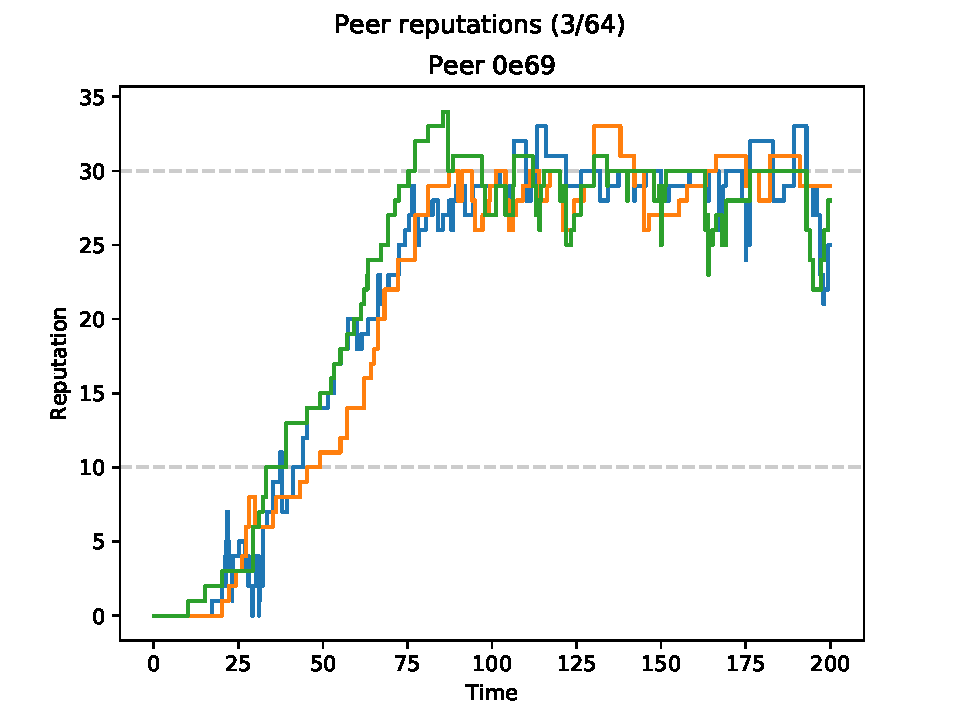
\includegraphics[width=0.5\columnwidth]{figures/expectations_off_no_att_high_buf_peer_reps_3_of_64}%
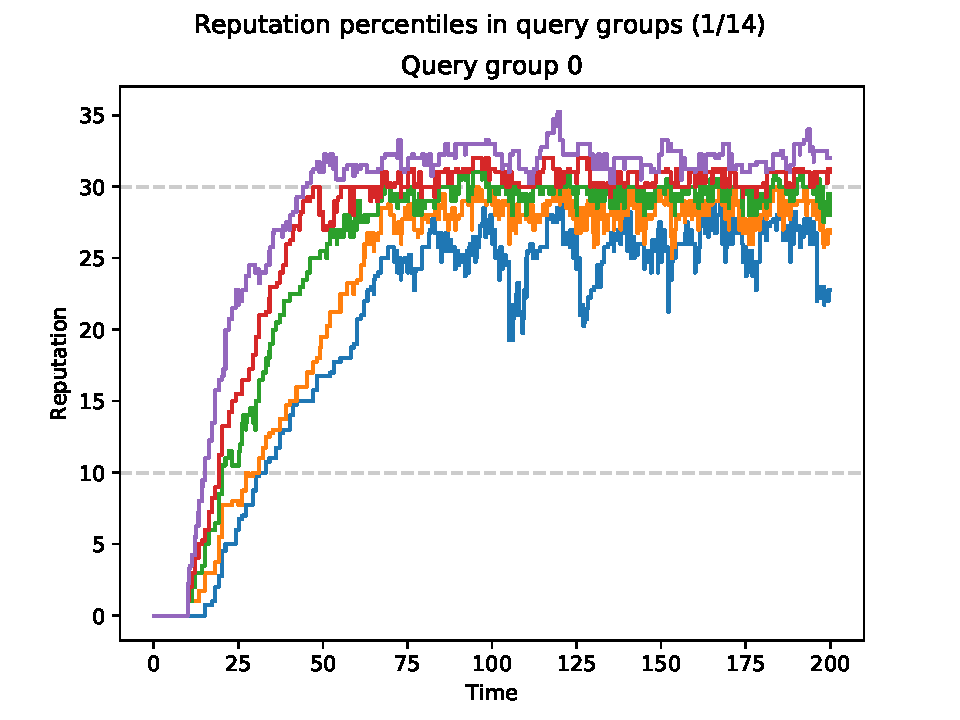
\includegraphics[width=0.5\columnwidth]{figures/expectations_off_no_att_high_buf_rep_percs_1_of_14}
\captionsettings{Reputation oscillation at a higher base level with increased
reputation buffer of
20}{penalty\_expectations/expectations\_off\_no\_att\_high\_buf.settings}
\label{fig:penalty_expectations_off_no_att_high_buf_peer_reps_percs}
\end{figure}

A workaround for this is to increase peer's reputation buffers. The result is
shown in
figure~\ref{fig:penalty_expectations_off_no_att_high_buf_peer_reps_percs}, where
the buffer has been increased from 4 to 20, meaning peers only let queries time
out once they have accumulated 30 reputation, rather than 14. Both peer
reputations and percentiles look similar, but have been shifted to a higher
level. Peers' reputations still fluctuate, but because of the higher buffer
doesn't dip below the no-penalty reputation (TODO terminology) of 10 anymore.

However, this is not a good solution because the amount of buffer a peer needs
is dependent on the amount of queries he is likely to receive at the same time,
i.e. within the time between letting the first query time out or sending a fail
response (TODO terminology) and the corresponding penalty arriving. Peers would
need to adjust the buffer based on the activity in the query group. Some
strategies for reputation attenuation presented in section~\ref{sec:attenuation}
also make it more difficult to gain reputation for a peer the more he already
has, so he may have to do much more work than necessary.

The better solution to the problem is to make peers expect to receive a penalty
when they do something they know is going to be penalized, and make their
decisions based on their reputation with expected penalties already applied. In
the implementation, peers make these expectations when they purposefully let a
query time out, and when they send a fail response (TODO terminology).

The expectations must themselves have a timeout, so that they can be removed in
case the peer who was expected to apply a penalty doesn't do so. This could
happen if either peer leaves the query group after the expectation has been
stored.

The implementation actually isn't ideal, as peers cannot expect timeout
penalties due to the recursive query problem (TODO terminology): When Alice
queries Bob, Bob may need to query Charlie in order to serve the query. If that
second query to Charlie takes so long that Alice's query times out, ideally Bob
would expect a timeout penalty. However, this is not implemented, and expecting
a penalty once the response from Charlie arrives doesn't make sense, since at
that point the penalty has likely already been applied.

\begin{figure}[t]
\centering
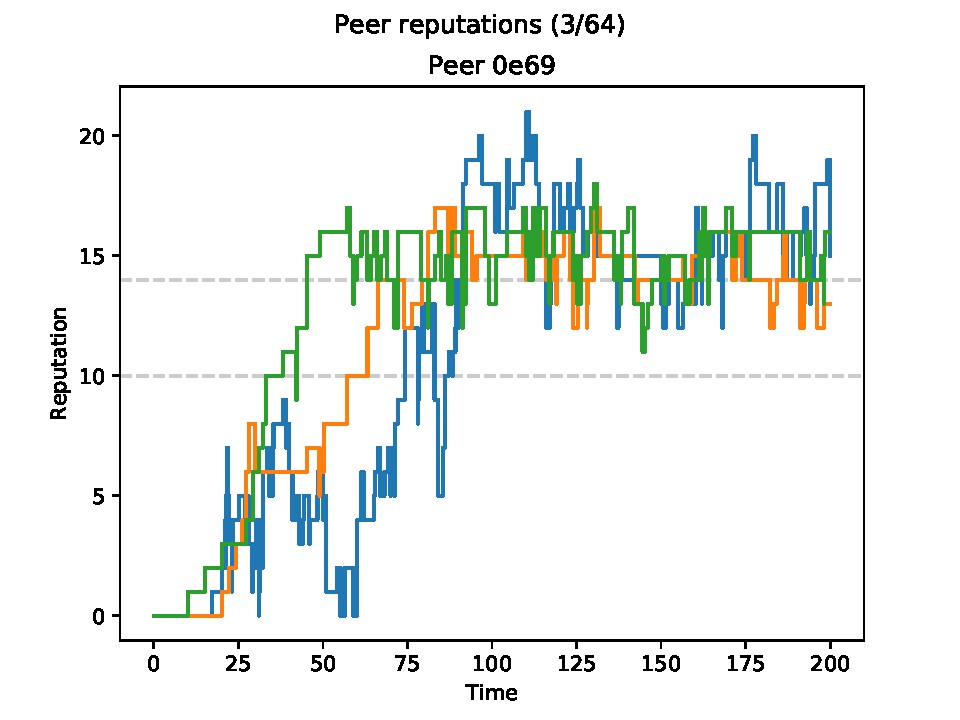
\includegraphics[width=0.5\columnwidth]{figures/expectations_on_no_att_peer_reps_3_of_64}%
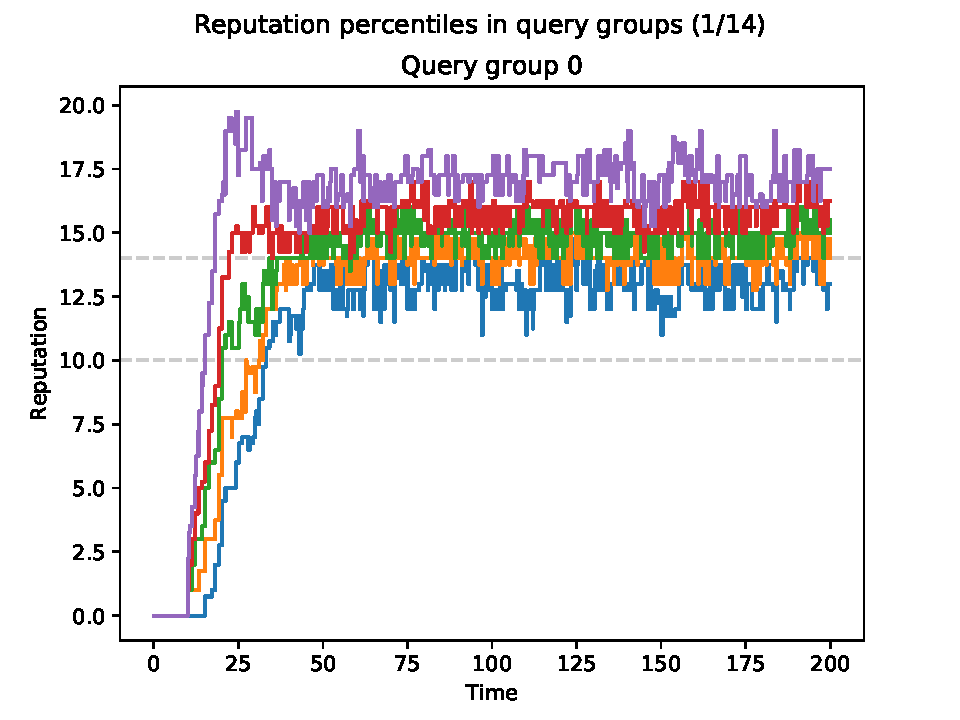
\includegraphics[width=0.5\columnwidth]{figures/expectations_on_no_att_rep_percs_1_of_14}
\captionsettings{Reduced reputation oscillation with expectations enabled, but
attenuation still
disabled}{penalty\_expectations/expectations\_on\_no\_att.settings}
\label{fig:penalty_expectations_on_no_att_peer_reps_percs}
\end{figure}

Figure~\ref{fig:penalty_expectations_on_no_att_peer_reps_percs} shows the result
of enabling penalty expectations, while reputation attenuation is still
disabled. Peers are now able to stay above the no-penalty reputation (TODO
terminology) without a large buffer.

To clarify, enabled penalty expectations are part of the default settings and
were used in the other simulations in this chapter.

\subsection{Impact of Attenuation}
Keeping penalty expectations disabled but enabling reputation attenuation also
significantly improves the behavior of the system.

\begin{figure}[t]
\centering
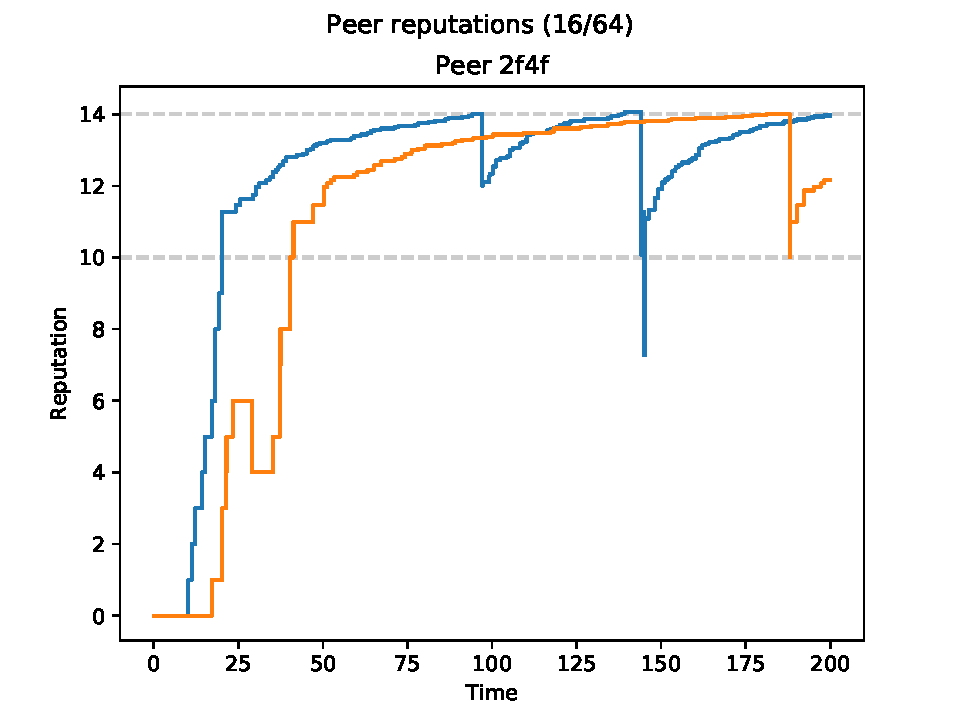
\includegraphics[width=0.5\columnwidth]{figures/expectations_off_peer_reps_16_of_64}%
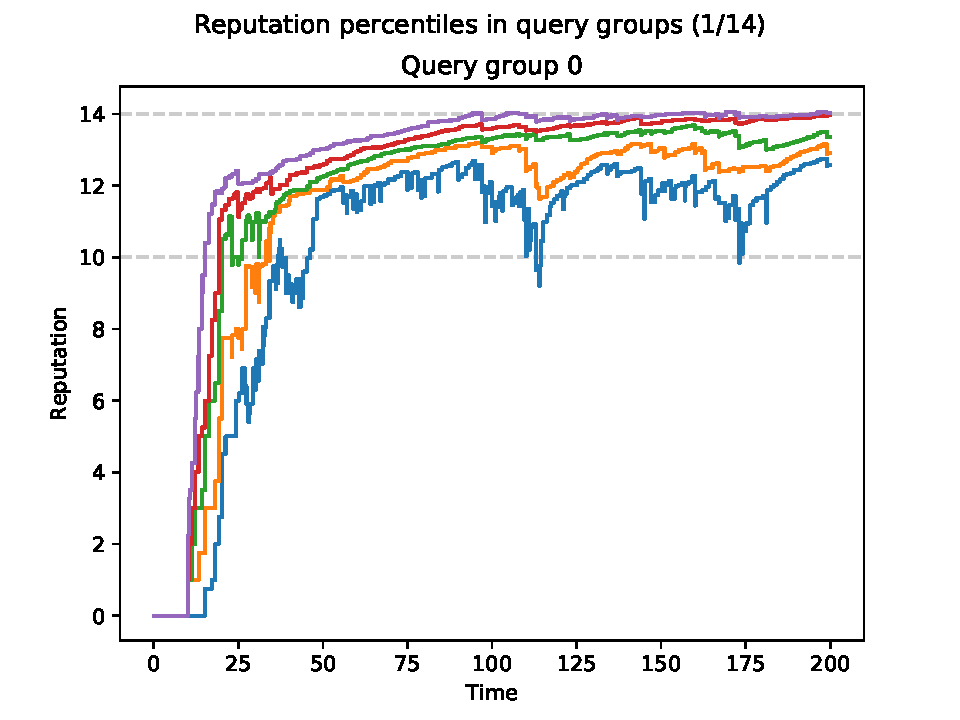
\includegraphics[width=0.5\columnwidth]{figures/expectations_off_rep_percs_1_of_14}
\captionsettings{Reputation of one peer and percentiles of a query group with
just attenuation enabled, expectations
off}{penalty\_expectations/expectations\_off.settings}
\label{fig:penalty_expectations_off_peer_reps_percs}
\end{figure}

Figure~\ref{fig:penalty_expectations_off_peer_reps_percs} gives an example of
this. The reputation percentiles of the query group selected for it show almost
all peers of the query group managing to stay above the no-penalty reputation
(TODO terminology) almost all of the time. At first glance this suggests that
penalty expectations are unnecessary if reputation attenuation is enabled.
However, the problem solved by penalty expectations still exists when just
attenuation is used: the individual reputations of the peer on the left show him
dipping below the no-penalty reputation (TODO terminology) just after he became
reputation saturated.

Rather, the reason just adding attenuation already looks a lot more tidy is that
it takes peers a lot longer to become reputation saturated. These are the
trigger points when peers without expectations let more queries time out than
they should. With fewer of them, peers don't lose reputation as often, making
their reputation much more stable.

Furthermore, reputation attenuation significantly reduces the number of timeouts
and thereby the number of queries (since timed out queries are retried). This
reduces, on average, the number of queries a peer lets time out before he
realizes he has dropped below the reputation at which he is saturated (TODO
confirm).

\section{Reputation Attenuation}
\label{sec:attenuation}
An important performance characteristic of the \ac{DHT} which the reputation
system supports is the likelihood that a peer responds to a query. Since we're
assuming all peers are selfish and inherently lazy, this is by no means
guaranteed.

The implementation models the peer behavior in such a way that peers do their
best to cooperate (i.e. respond to queries) until they reach the no-penalty
reputation plus a buffer (TODO term for this, e.g. no-work reputation? also for
expectation section) to be able to tolerate trembles, which in the default
settings are 10 and 4, respectively. (TODO the following is probably just a
recap by now. necessary?) That means peers play nice and gather reputation until
they have 14, then decide that they have enough. The next time they're required
to do something, e.g. respond to a query, they ignore this, incurring a penalty.
This puts them below their no-work reputation and they cooperate again until
they reach it again.

The amount of good deeds (TODO terminology, there should be a term for
reward-worthy actions as well as penalty-worthy ones) a peer has to perform to
get back up to the no-work reputation (TODO terminology) ultimately determines
his response probability. It is determined by the magnitude of the penalty he
receives when he drops below his no-work reputation (TODO terminology) and that
of the rewards he receives as he works his way back up (TODO this is phrased
abstractly as good and bad deeds, but the only relevant things implemented are
successful responses and timeouts. make it concrete?). So the response
probability of the system can be adjusted via the penalties and rewards, with $1
- \frac{reward}{penalty} = response probability$ (TODO do this properly, define
response/timeout prob).

However, this assumes that all peers are already above the no-penalty reputation
(TODO terminology) and well-established in the system. But the larger the
difference between reward and penalty is, the more difficult it becomes for a
newcomer to the system to become established (TODO ref becoming established
section). It also assumes that trembles happen relatively rarely, since
otherwise peers may be unlucky and tremble repeatedly without being able to make
up for it in between, crashing their reputation. The recursive query problem
(TODO terminology) may make it impossible for newcomers to become established.,
For example, assuming a target response probability of 95\%, the ratio of reward
to penalty would have to be 1:20, so newcomers would have to earn more than 20
rewards for every penalty they incur in order to make progress towards the
no-penalty reputation (TODO terminology).

Removing the no-penalty reputation (TODO terminology)(i.e. setting it to 0) is
also not an option, since the purpose of it is to prevent whitewashing by
requiring newcomers to put in some work before enjoying unpenalized service. The
solution presented here is to make a distinction between these two phases,
establishing oneself in the system while having less than the no-penalty
reputation (TODO terminology), and the steady state after. In the former,
reputation is gained as usual, but in the latter, reputation earnings are
attenuated by one of three strategies in a way that allows to regulate the
response probability without impacting newcomers' ability to establish
themselves.

A distinction is made between \emph{raw reputation} $r_r$ and \emph{effective
reputation} $r_e$, where \emph{raw reputation} is the reputation as previously,
and \emph{effective reputation} is the result of applying an attenuation
function $att$ to the raw reputation. The effective reputation is what is used
when a decision has to be made based on a peer's reputation, e.g. how much of a
penalty delay (TODO terminology) to impose.

When updating a peer's reputation, rewards are applied to the raw reputation,
while penalties are applied to the effective reputation:

When a reward, i.e. a reputation update changing the reputation by an amount
$r_{diff} > 0$, is applied to a peer with effective reputation $r_e$, the
effective reputation is set to $att(att^{-1}(r_e) + r_{diff})$. I.e., the raw
reputation is calculated from the effective reputation, then the update applied,
and the result turned into effective reputation.

When a penalty, i.e. a reputation update changing the reputation by an amount
$r_{diff} < 0$, is applied to a peer with effective reputation $r_e$, the
effective reputation is set to $r_e - r_{diff}$.

With these differing rules for rewards and penalties it is possible to make it
increasingly harder for peers to gain effective reputation the more they already
have, while maintaining the same threat for misbehavior.

In all of the strategies, there is an \emph{attenuation threshold}, which is the
amount of reputation below which reputation is unmodified, i.e. $att$ is the
identity function for input values below the threshold. The threshold by default
is the no-penalty reputation. An upper limit on the reputation which peers can't
surpass is also implemented, but has no influence since peers don't reach it in
the simulations.

\subsection{Strategy: \emph{Constant}}
The first strategy simply multiplies all raw reputation above the threshold by a
fixed coefficient $c$. $t$ is the reputation threshold, $l$ the upper reputation
limit.

\[att_{const}(r_r) = min(min(r_r, t) + c \cdot max(r_r - t, 0), l)\]

\begin{figure}[t]
\centering
\begin{tikzpicture}
\begin{axis}[
    xlabel=$r_r$,
    ylabel={$att_{const}(r_r)$},
    xmin=0,
    xmax=75,
    ymin=0,
    ymax=20
]
\addplot[domain=0:75, samples=76]{min(min(x, 10) + 0.08 * max(x - 10, 0), 15)};
\end{axis}
\end{tikzpicture}
\caption{Raw vs. effective reputation for \emph{constant} attenuation ($t$ = 10,
$c = 0.08$, $l = 15$)}
\label{fig:att_const_raw_vs_eff}
\end{figure}

\subsection{Strategy: \emph{Exponential}}
This strategy raises all raw reputation above the threshold to a fixed power $p$
and multiplies the result by a coefficient $c$. $t$ is the reputation threshold,
$l$ the upper reputation limit.

\[att_{exp}(r_r) = min(min(r_r, t) + c \cdot max(r_r - t, 0)^p, l)\]

\begin{figure}[t]
\centering
\begin{tikzpicture}
\begin{axis}[
    xlabel=$r_r$,
    ylabel={$att_{exp}(r_r)$},
    xmin=0,
    xmax=75,
    ymin=0,
    ymax=20
]
\addplot[domain=0:75, samples=751]{min(min(x, 10) + max(x - 10, 0) ^ 0.35, 15)};
\end{axis}
\end{tikzpicture}
\caption{Raw vs. effective reputation for \emph{exponential} attenuation ($t$ =
10, $p = 0.35$, $c = 1$, $l = 15$)}
\label{fig:att_exp_raw_vs_eff}
\end{figure}

\subsection{Strategy: \emph{Harmonic}}
In this strategy, attenuation is done above the threshold by a coefficient that
is harmonically decreasing. $a$ and $k$ are parameters, $t$ is the reputation
threshold, $l$ the upper reputation limit.  Essentially, raw reputation in the
interval $[t + i, t + i + 1], i \in \mathbb{N}$ is attenuated by the coefficient
$\frac{1}{a + i \cdot k}$.

\[att_{harm}(r_r) = min(min(r_r, t) + \sum_{i=0}^{\lceil r_r
\rceil}{min(\frac{u(max(r_r - t, 0), i)}{a + i \cdot k}, 1)}, l)\]

Here, $u$ is a function giving the amount of raw reputation above the threshold
that has not been "used up" by "converting" raw to effective reputation in the
interval $[t, i]$:

\[u(r_r, m) = max(r_r - \sum_{i=0}^m{a + i \cdot k}, 0)\]

For example, with $a = 1$, $k = 8$ and $t = 10$, a peer needs 1 raw reputation
to get from 10 to 11, 9 to get from 11 to 12, 17 to get from 12 to 13, 8.5 to
get from 12 to 12.5 etc.

\begin{figure}[t]
\centering
\begin{tikzpicture}
\begin{axis}[
    xlabel=$r_r$,
    ylabel={$att_{harm}(r_r)$},
    xmin=0,
    xmax=75,
    ymin=0,
    ymax=20
]
\addplot[domain=0:75, samples=751] coordinates {
    (0, 0)
    (11, 11)
    (20, 12)
    (37, 13)
    (52, 14)
    (85, 15)
};
\end{axis}
\end{tikzpicture}
\caption{Raw vs. effective reputation for \emph{harmonic} attenuation ($t$ = 10,
$a = 1$, $k = 8$, $l = 15$)}
\label{fig:att_harm_raw_vs_eff}
\end{figure}

\subsection{Comparison}
Figures~\ref{fig:attenuation_percs} and \ref{fig:attenuation_resp} show
reputation percentiles and response statuses of simulation runs demonstrating
the different attenuation strategies. The percentiles are all of the same query
group, with the same members (TODO confirm). The example was chosen to
illustrate a few points. It is not representative of the overall performance
(TODO confirm, quantify), many other groups perform better.

The parameters in the attenuated simulations have been chosen so that it takes
roughly the same amount of raw reputation to get from 10 (the attenuation
threshold) to 14 (the saturation reputation for all peers): $\frac{4}{0.08} =
50$ for \emph{constant}, $4^{\frac{1}{0.35}} \approx 52.5$ for
\emph{exponential}, and $1 + 9 + 17 + 25 = 52$ for \emph{harmonic}. In effect,
the first peers to become saturated in the attenuated cases do so at around the
same time.

\begin{figure}[t]
  \centering
  \begin{subfigure}[t]{0.45\columnwidth}
    \centering
    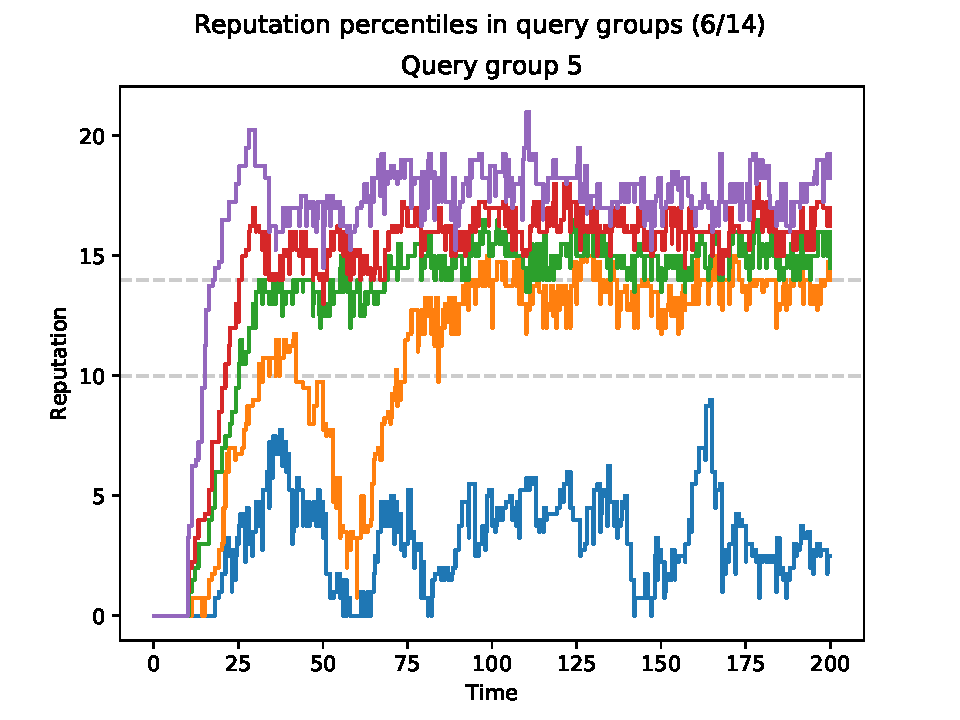
\includegraphics[width=\columnwidth]{figures/attenuation_no_attenuation_rep_percs_6_of_14}
    \subcaptionsettings{No
    attenuation}{attenuation/attenuation\_no\_attenuation.settings}
    \label{fig:attenuation_no_att_percs}
  \end{subfigure}\hfill%
  \begin{subfigure}[t]{0.45\columnwidth}
    \centering
    \includegraphics[width=\columnwidth]{figures/{{attenuation_0.08_constant_rep_percs_6_of_14}}}
    \subcaptionsettings{\emph{Constant} attenuation, $c =
    0.08$}{attenuation/attenuation\_0.08\_constant.settings}
    \label{fig:attenuation_constant_percs}
  \end{subfigure}\hfill\\%
  \begin{subfigure}[t]{0.45\columnwidth}
    \centering
    \includegraphics[width=\columnwidth]{figures/{{attenuation_0.35_1_exponential_rep_percs_6_of_14}}}
    \subcaptionsettings{\emph{Exponential} attenuation, $p = 0.35$, $c =
    1$}{attenuation/attenuation\_0.35\_1\_exponential.settings}
    \label{fig:attenuation_exp_percs}
  \end{subfigure}\hfill%
  \begin{subfigure}[t]{0.45\columnwidth}
    \centering
    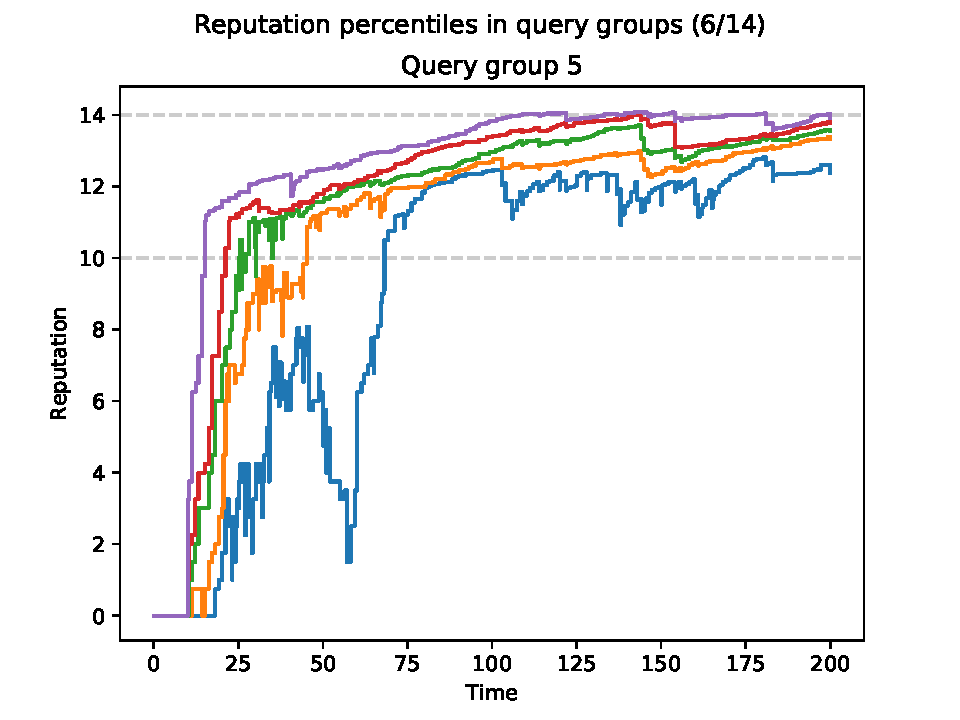
\includegraphics[width=\columnwidth]{figures/attenuation_1_8_harmonic_rep_percs_6_of_14}
    \subcaptionsettings{\emph{Harmonic} attenuation, $a = 1$, $k =
    8$}{attenuation/attenuation\_1\_8\_harmonic.settings}
    \label{fig:attenuation_harmonic_percs}
  \end{subfigure}
  \caption{Reputation percentiles in the same query group for different
  attenuation strategies. For all, $t = 10$ and $l = 15$.}
  \label{fig:attenuation_percs}
\end{figure}

In the case of no attenuation (figure~\ref{fig:attenuation_no_att_percs}) the
5th percentile doesn't make it above the no-penalty reputation. This is due to
one peer\footnote{Since this query group contains 16 peers, the 5th percentile
is just the one peer.} (TODO peer id 8961) who is suffering from the recursive
query problem (TODO terminology). Over the course of the simulation, he receives
140 penalties, all of them for timeouts. There are also 132 responses sent by
him that were unmatched at the receiver (TODO late instead of unmatched, if that
gets implemented), meaning they were sent after the timeout was triggered at the
receiver. So the peer tried, but was frequently too late (TODO confirm by
archiving timed out queries and implementing a metric measuring how many
too-late recursive queries there are).

This peer is not struggling in the cases with attenuation turned on. The likely
reason is that, during recursive queries he is experiencing more timeouts
without attenuation than with attenuation (TODO confirm this is the only
reason). Without it, it is much easier for the other peers to become reputation
saturated.

Without attenuation, some oscillation can be seen in the reputation percentiles,
which reflects oscillation in individual peer reputations. Peers are also
getting significantly above the reputation at which they are saturated (14). The
reason is that, while peers expect penalties (see
section~\ref{sec:penalty_expectations}), they do not expect rewards. This leads
to them answering multiple queries in a row, even though answering only the
first would have made them saturated; the reputation update simply hasn't
arrived yet.  This is of course still true for the attenuated cases, but here it
takes a lot more raw reputation to get to the saturated effective reputation.

There is no discernible difference between \emph{exponential} and
\emph{harmonic} attenuation, which makes sense considering their similarity in
the relationship between raw and effective reputation
(figures~\ref{fig:att_exp_raw_vs_eff} and \ref{fig:att_harm_raw_vs_eff}).

There is some difference between them and \emph{constant}, however. In the
latter, every point of raw reputation is attenuated in the same way, while in
the former the attenuation rises as the peer's accumulated effective reputation
rises. For \emph{harmonic}, the first point above the attenuation threshold is
not attenuated at all, for \emph{exponential}, attenuation just above the
threshold is actually negative, i.e. the effective reputation yielded is greater
than the raw reputation. This makes it easier for peers to gain reputation just
above the no-penalty reputation (TODO terminology) in order to be able to
tolerate a tremble. This is demonstrated by the simulations: the 5th percentile
(the struggling peer) manages to reliably stay above the no-penalty reputation
with \emph{exponential} or \emph{harmonic} attenuation
(figures~\ref{fig:attenuation_exp_percs} and
\ref{fig:attenuation_harmonic_percs}), while he dips below it once more for the
\emph{constant} case (figure~\ref{fig:attenuation_constant_percs}). And the 25th
percentile is also "stuck" at around the no-penalty reputation (TODO
terminology) for a lot longer in the \emph{constant} case.

\begin{figure}[t]
\centering
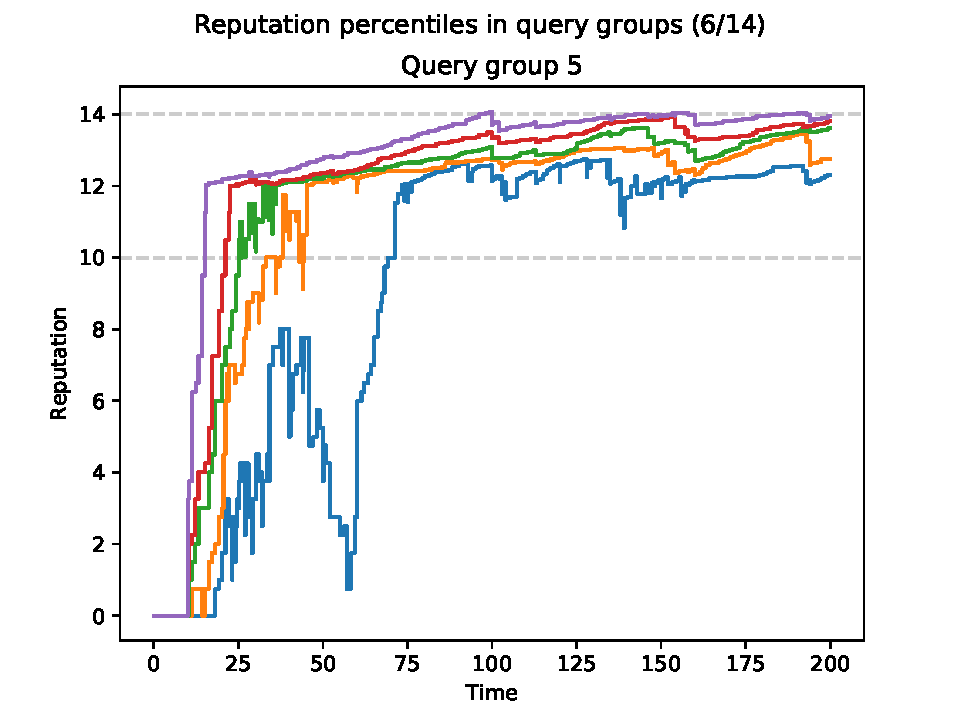
\includegraphics[width=1\columnwidth]{{{figures/attenuation_0.0417_constant_12_threshold_rep_percs_6_of_14}}}
\captionsettings{Reputation percentiles over time for \emph{constant}
attenuation with higher threshold ($c = 0.0417$, $t =
12$)}{attenuation/attenuation\_0.0417\_constant\_12\_threshold.settings}
\label{fig:attenuation_0.0417_constant_12_threshold_percs}
\end{figure}

A possibility to address this is to set the attenuation threshold above the
no-penalty reputation, allowing peers to e.g. to gain enough reputation to
tolerate a tremble without attenuation kicking in. This is shown in
figure~\ref{fig:attenuation_0.0417_constant_12_threshold_percs}: \emph{constant}
attenuation is used but the threshold is set to 12, and the coefficient is
adjusted to 0.0417, so that it still takes 50 raw reputation to get from 10 to
14 effective reputation. The struggling peer's reputation develops in a way
comparable to \emph{exponential} or \emph{harmonic} from
figure~\ref{fig:attenuation_percs}.

A potential problem with this approach is that the rules of the system must make
an assumption about how many trembles a peer should be able to tolerate and set
the attenuation threshold appropriately. In order to achieve the same expected
response probability, effective reputation above the higher threshold has to be
more "expensive". However, if some peer is satisfied with being able to tolerate
fewer trembles than the system assumes, he may get away with no attenuation at
all. In the example shown in
figure~\ref{fig:attenuation_0.0417_constant_12_threshold_percs}, the threshold
is set so peers can easily get to 12 reputation, where they are able to tolerate
one penalty of 2 points. A peer may be confident he won't drop below 10
reputation once he reaches it, and let queries time out once he reaches 12
reputation. That peer would never have his reputation attenuated and have a very
low response probability.

On the other hand, \emph{exponential} and \emph{harmonic} attenuation are
disadvantageous for peers wishing to be able to tolerate more trembles for extra
reliability, since effective reputation gets more and more expensive. For
example, using \emph{exponential} attenation with $c = 1$, $p = 0.35$ (as in the
examples), it takes about 52.5 raw reputation to get from 10 to 14 effective
reputation. In order to get from 10 to 16 (being able to tolerate 3 trembles),
it takes 167.2. This puts a much higher stress on such peers wishing for more
reliability.

A solution to this could be to cap the "cost" of effective reputation,
essentially combining \emph{exponential} or \emph{harmonic} attenuation with
\emph{constant} attenuation, switching over to the latter once a certain amount
of effective reputation has been earned.

The reputation cap (the upper limit of effective reputation that can't be
surpassed) is meant to ensure activity in the query groups by preventing peers
from collecting a lot of reputation up front and then not responding to queries
for prolonged periods. In the simulations, this didn't become relevant because
all peers let queries time out once 14 effective reputation are reached.  With
\emph{exponential} or \emph{harmonic} attenuation, it's not a viable strategy
anyway, since effective reputation gets more and more "expensive". But with
\emph{constant} attenuation an upper limit may well become necessary.

\begin{figure}[t]
  \centering
  \begin{subfigure}[t]{0.45\columnwidth}
    \centering
    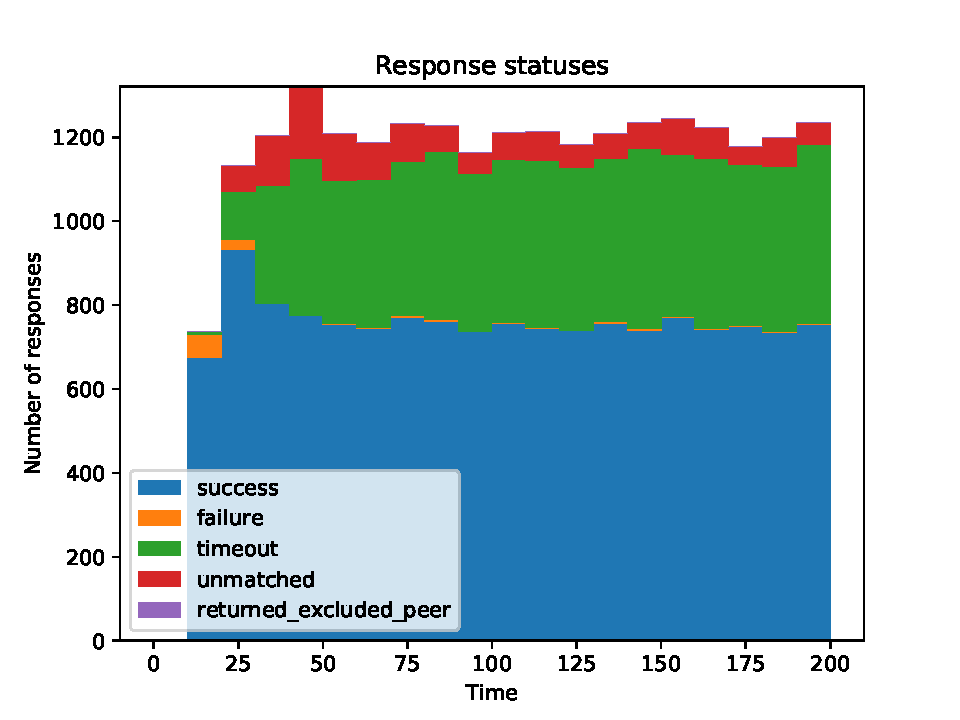
\includegraphics[width=\columnwidth]{figures/attenuation_no_attenuation_resp_statuses}
    \subcaptionsettings{No
    attenuation}{attenuation/attenuation\_no\_attenuation.settings}
    \label{fig:attenuation_no_att_resp}
  \end{subfigure}\hfill%
  \begin{subfigure}[t]{0.45\columnwidth}
    \centering
    \includegraphics[width=\columnwidth]{figures/{{attenuation_0.08_constant_resp_statuses}}}
    \subcaptionsettings{\emph{Constant} attenuation, $c =
    0.08$}{attenuation/attenuation\_0.08\_constant.settings}
    \label{fig:attenuation_constant_resp}
  \end{subfigure}\hfill\\%
  \begin{subfigure}[t]{0.45\columnwidth}
    \centering
    \includegraphics[width=\columnwidth]{figures/{{attenuation_0.35_1_exponential_resp_statuses}}}
    \subcaptionsettings{\emph{Exponential} attenuation, $p = 0.35$, $c =
    1$}{attenuation/attenuation\_0.35\_1\_exponential.settings}
    \label{fig:attenuation_exp_resp}
  \end{subfigure}\hfill%
  \begin{subfigure}[t]{0.45\columnwidth}
    \centering
    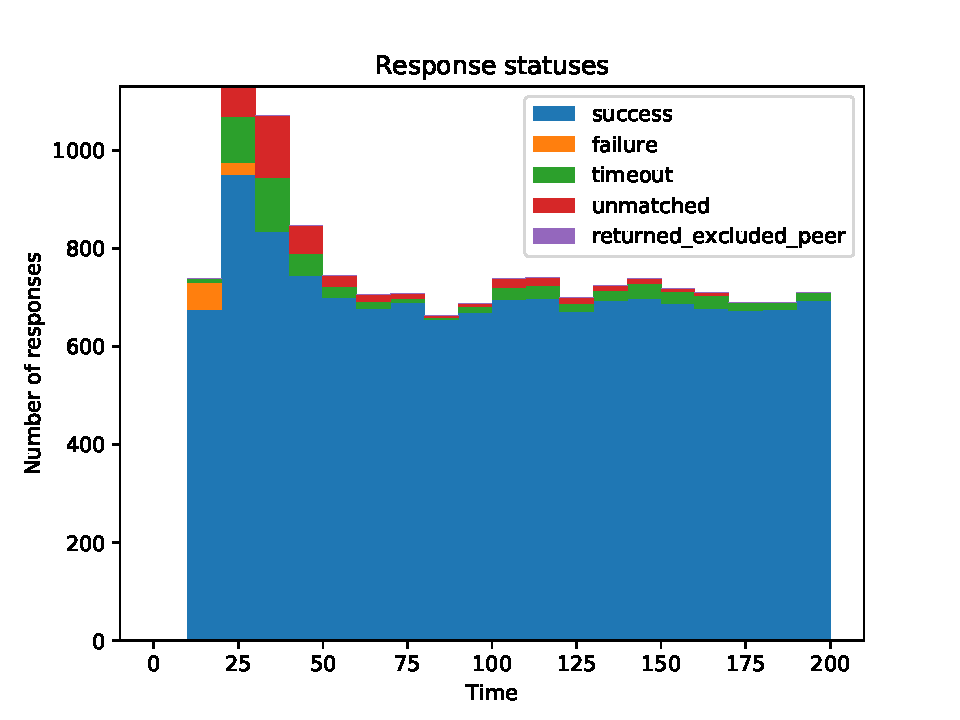
\includegraphics[width=\columnwidth]{figures/attenuation_1_8_harmonic_resp_statuses}
    \subcaptionsettings{\emph{Harmonic} attenuation, $a = 1$, $k =
    8$}{attenuation/attenuation\_1\_8\_harmonic.settings}
    \label{fig:attenuation_harmonic_resp}
  \end{subfigure}
  \caption{Response statuses for different attenuation strategies. For all, $t =
  10$ and $l = 15$.}
  \label{fig:attenuation_resp}
\end{figure}

Figure~\ref{fig:attenuation_resp} shows the response statuses for the
simulations corresponding to the reputation percentiles in
figure~\ref{fig:attenuation_percs}. Again, there is virtually no difference
between \emph{exponential} and \emph{harmonic} attenuation. Both yield good
performance with a low percentage of timeouts. It matches (TODO confirm, do the
math) the theorectical response probability given that peers let queries time
out once they reach 14 reputation, take a penalty of 2 points and then work
their way back up to 14. (TODO give numbers, maybe a table with number of
responses, timeouts?).

\emph{Constant} attenuation is very similar, but has a few more timeouts. This
is due to the fact that it takes less raw reputation to get from 12 to 14 than
for the other attenuation strategies (25 compared to 45.26 and 42,
respectively). That means after letting an incoming query time out, peers can
work their way back up to 14 faster (TODO confirm theoretical prediction holds,
give numbers, table?).

Without attenuation, there are many more timeouts, and as a consequence also
many more messages in total (TODO give numbers, confirm theoretical prediction
holds). Here, peers are very easily able to earn 14 reputation and become
saturated, at which point they let the next query time out. This is the reason
attenuation is necessary.

\begin{figure}[t]
\centering
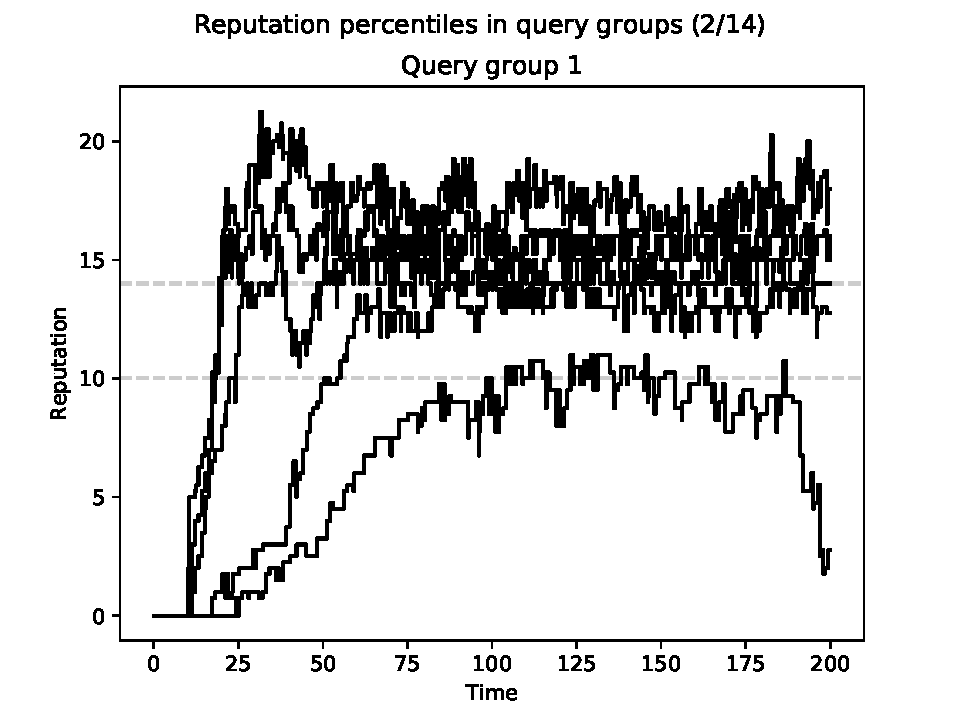
\includegraphics[width=1\columnwidth]{figures/attenuation_no_attenuation_selection_overlap_rep_percs_2_of_14}
\captionsettings{Reputation percentiles over time with no attenuation and peer
selection strategy \emph{overlap} in one query
group}{attenuation/attenuation\_no\_attenuation\_selection\_overlap.settings}
\label{fig:attenuation_no_att_selection_overlap_rep_percs}
\end{figure}

Figure~\ref{fig:attenuation_no_att_selection_overlap_rep_percs} shows reputation
percentiles with no attenuation and the peer selection strategy \emph{overlap}.
The same settings were used and the same query group shown as in
figure~\ref{fig:selection_overlap_rep_percs} from section~\ref{sec:selection}
covering selection strategies, except that attenuation has been turned off
(previously, the default \emph{exponential} attenuation was used).

The comparison shows that the problem of the \emph{overlap} peer selection
strategy where some peers are unlucky and are only sent queries with low
priority is less severe when attenuation is turned off. This is because the
"lucky" peers who are preferred query recipients are reputation saturated after
much less time and letting their incoming queries time out, at which point the
"unlucky" peers are chosen. The fundamental problem still exists though, the
"unlucky" peers still have to wait.

\section{Query Group Reevaluation}
\label{sec:rep_avail_group_reeval}
- incomplete implementation causes problems: peers first find their necessary
  query peers, but then they leave. potentially mitigated by running query peer
  discovery repeatedly now?

\section{Bootstrapping}
\label{sec:rep_avail_bootstrapping}
\subsection{Bootstrapping an Empty Network}
\subsection{Becoming Establised in a Running System}
- number of introductions needed to get subprefix coverage

\section{Effect of Small Sync Groups}
- with small sync groups, particularly one peer per sync group, the system is
  very brittle, even if all sync groups exist (see 11/about)
- routing loops are a problem that can occur when overlap isn't the first
  selection criterion (particularly subprefix queries). this can lead to
  timeouts and lots of penalties (related to brittleness with small sync groups)
- the problem with each peer in his own sync group is apparently that, once the
  first peers reach 14, they let queries time out, and this causes problems to
  other peers who were relying on them, crashing reputations. with longer
  routing prefixes and deeper lookups (more hops), the likelihood of something
  timing out on the way rises.

\section{Stuff that hasn't been looked into (TODO section name)}
- making the relationship between reputation and penalty delay non-proportional

\section{Large Simulation (TODO section name)}
- TODO just do the whole thing with the "best" settings with at least 1024 peers


-----------------------
- recursive-query-problem, observable in peer reputations (some configurations?
  see 8/about)
- impact of query group size
- uneven distribution of rep (effect of even sync groups)
- difference in expected delays because of difference in time between
  calculating; may have changed in the meantime
- peers can get more than their maximum desired reputation
- in the case of multiple shared groups, where do peers get rep?
- query peer selection: must send to peer with lowest rep
- uneven query distribution
- query group reevaluation mechanism, caveat that new groups can't be created,
  only when a new peer is introduced
- missing sync groups are a problem: no one can say for sure that there doesn't
  exist a peer in that sync group, so peers querying for missing subprefix
  coverage give out penalties to those they query because of the resulting fail
  responses. no real solution other than ensuring non-empty sync groups (linked
  to replication). this is confirmed by giving peers global knowledge of which
  sync groups exist and not having them query for those subprefixes, then
  everything works. even one missing sync group can screw everything up (see 64
  peers/6 bit routing prefix case).
- number of introductions relative to the amount of peers has an effect on how
  easy it is for the system to get started (see 11/about)
